\documentclass[12pt,a4paper]{article}

% ── Packages ──
\usepackage[utf8]{inputenc}
\usepackage[T1]{fontenc}
\usepackage{mathptmx}                    % Times New Roman
\usepackage[margin=1in]{geometry}
\usepackage{setspace}
\usepackage{graphicx}
\usepackage{booktabs}
\usepackage{caption}
\usepackage{subcaption}
\usepackage{float}
\usepackage{hyperref}
\usepackage{xcolor}
\usepackage{tabularx}
\usepackage{array}
\usepackage{longtable}
\usepackage{amsmath}
\usepackage{natbib}
\usepackage{titlesec}
\usepackage{fancyhdr}
\usepackage{enumitem}

% ── Formatting ──
\setstretch{1.15}
\hypersetup{colorlinks=true,linkcolor=blue!60!black,citecolor=blue!60!black,urlcolor=blue!60!black}
\titleformat{\section}{\normalfont\Large\bfseries}{\thesection.}{0.5em}{}
\titleformat{\subsection}{\normalfont\large\bfseries}{\thesubsection}{0.5em}{}
\titleformat{\subsubsection}{\normalfont\normalsize\bfseries}{\thesubsubsection}{0.5em}{}
\pagestyle{fancy}
\fancyhf{}
\rhead{\small LULC Exposure Analysis -- Maharashtra}
\lhead{\small CM801 -- Climate Studies Risk Analysis}
\cfoot{\thepage}
\renewcommand{\headrulewidth}{0.4pt}

% ══════════════════════════════════════════════════════════════
\begin{document}

% ── Cover Page ──
\begin{titlepage}
\centering
\vspace*{1cm}
{\Large \textbf{Indian Institute of Technology Bombay}}\\[0.3cm]
{\large CM801 -- Climate Studies Risk Analysis}\\[0.2cm]
{\large Spring Semester 2025--26}\\[1.5cm]

\rule{\textwidth}{1.5pt}\\[0.5cm]
{\LARGE \textbf{Spatial Mapping of Land Use and Land Cover (LULC) Exposure in Maharashtra:}}\\[0.3cm]
{\LARGE \textbf{A Gridded and District-Level Analysis}}\\[0.5cm]
\rule{\textwidth}{1.5pt}\\[2cm]

{\large \textbf{Group Members and Contributions}}\\[0.5cm]

\begin{tabular}{|l|c|p{6cm}|}
\hline
\textbf{Name} & \textbf{Roll Number} & \textbf{Contribution} \\
\hline
Nawang Tashi   & 2360760 & Data acquisition, literature review, and LULC classification validation \\
\hline
Shourya Goyal  & 2360733 & District-level zonal analysis, choropleth mapping, and statistical interpretation \\
\hline
Rushabh Bonde  & 2360703 & Gridded spatial analysis, heatmap generation, and GIS processing \\
\hline
Sajjad Nakhwa  & 2360702 & Climate risk exposure index computation and temporal change detection \\
\hline
Tushar Bajaj   & 23B2107 & Multi-tile raster reprojection and mosaicking pipeline, Climate Risk Exposure Index formulation, and geospatial visualization design \\
\hline
\end{tabular}

\vfill
{\large \textbf{Date:} April 5, 2026}
\end{titlepage}

% ══════════════════════════════════════════════════════════════
\section{Introduction and Study Area}
% ══════════════════════════════════════════════════════════════

Land Use and Land Cover (LULC) is a fundamental descriptor of the Earth's surface that directly influences climate vulnerability, ecological resilience, and socio-economic exposure \citep{foley2005global}. Understanding the spatial distribution and temporal dynamics of LULC is essential for assessing how populations, infrastructure, and ecosystems are exposed to climate-related hazards such as droughts, floods, urban heat islands, and loss of carbon sequestration capacity \citep{ipcc2022}.

Maharashtra, India's third-largest state by area ($\sim$307,713~km\textsuperscript{2}) and second-most populous ($\sim$124 million), extends from 15\textdegree36'N to 22\textdegree06'N and 72\textdegree36'E to 80\textdegree54'E. The state encompasses diverse landscapes---from the densely urbanized Mumbai Metropolitan Region to the drought-prone Marathwada plateau, from the forested Western Ghats to the semi-arid Vidarbha region \citep{maharashtra2023}. This topographic diversity drives strong rainfall gradients (400~mm in Marathwada to over 6,000~mm in the Western Ghats), shaping agricultural practices, forest distribution, and urbanization patterns \citep{gadgil1992western}.

This project leverages the ESRI 2024 and 2017 Sentinel-2 LULC datasets \citep{karra2021global} to conduct a comprehensive spatial analysis of land cover exposure across Maharashtra at district and 25~km grid levels, synthesizing the results into a composite Climate Risk Exposure Index.

% ══════════════════════════════════════════════════════════════
\section{Objectives}
% ══════════════════════════════════════════════════════════════

\begin{enumerate}[leftmargin=2cm]
    \item To generate a high-resolution LULC map of Maharashtra for 2024 using ESRI Sentinel-2 10m land cover data.
    \item To quantify the spatial distribution of each LULC class at state, district, and gridded (25~km $\times$ 25~km) levels.
    \item To perform temporal change detection by comparing LULC distributions between 2017 and 2024.
    \item To develop a composite Climate Risk Exposure Index integrating agricultural exposure, urban exposure, forest buffer capacity, urbanization pressure, and deforestation trends.
    \item To identify and rank the most climate-vulnerable districts in Maharashtra.
\end{enumerate}

% ══════════════════════════════════════════════════════════════
\section{Data and Methodology}
% ══════════════════════════════════════════════════════════════

\subsection{Data Sources}

Table~\ref{tab:data_sources} summarizes the datasets used in this study.

\begin{table}[H]
\centering
\caption{Datasets used in the LULC exposure analysis.}
\label{tab:data_sources}
\begin{tabular}{p{3.5cm} p{3cm} p{3cm} p{4cm}}
\toprule
\textbf{Dataset} & \textbf{Source} & \textbf{Resolution} & \textbf{Description} \\
\midrule
ESRI Sentinel-2 LULC 2024 & Living Atlas \citep{esri2024} & 10 m & Tiles 43P, 43Q, 44Q; Jan--Dec 2024 \\
ESRI Sentinel-2 LULC 2017 & Living Atlas \citep{esri2024} & 10 m & Tiles 43P, 43Q, 44Q; Jan 2017--Jan 2018 \\
Maharashtra State Boundary & DataMeet \citep{datameet2023} & Vector & Admin Level 2 boundary \\
District Boundaries & DataMeet \citep{datameet2023} & Vector & Census 2011 district boundaries (35 districts) \\
\bottomrule
\end{tabular}
\end{table}

The ESRI 10m Annual Land Cover product is derived from Sentinel-2 multispectral imagery using a deep learning classification model trained on billions of labeled pixels. The classification scheme includes 9 land cover classes (Table~\ref{tab:lulc_classes}), with an overall global accuracy of approximately 85\% \citep{karra2021global}.

\begin{table}[H]
\centering
\caption{ESRI Sentinel-2 LULC classification scheme.}
\label{tab:lulc_classes}
\begin{tabular}{clp{8cm}}
\toprule
\textbf{Value} & \textbf{Class Name} & \textbf{Description} \\
\midrule
2  & Trees             & Woody vegetation $>$3m height; canopy cover $>$15\% \\
3  & Grass             & Open areas dominated by grasses, not tilled \\
4  & Flooded Vegetation & Areas of waterlogged vegetation (mangroves, marshes) \\
5  & Crops             & Cultivated areas with planted/harvested vegetation \\
6  & Scrub/Shrub       & Woody vegetation $<$3m height \\
7  & Built Area        & Human-made structures, impervious surfaces \\
8  & Bare Ground       & Rock, sand, soil with $<$10\% vegetation \\
9  & Snow/Ice          & Permanent and seasonal snow or ice \\
11 & Water             & Open water bodies, rivers, reservoirs \\
\bottomrule
\end{tabular}
\end{table}

\subsection{Methodology}

The analytical workflow comprises six stages:

\textbf{Stage 1: Data Preprocessing and Clipping.}
Three LULC GeoTIFF tiles (43P, 43Q in EPSG:32643; 44Q in EPSG:32644) were processed per year. The 44Q tile was reprojected to EPSG:32643 using nearest-neighbor resampling to preserve categorical LULC classes. All tiles were merged into a single mosaic using \texttt{rasterio.merge} in Python, then clipped to the Maharashtra state boundary (reprojected from WGS84 to UTM Zone 43N), yielding year-specific clipped rasters covering all 35 districts.

\textbf{Stage 2: State-Level LULC Statistics.}
Pixel counts per LULC class were computed from the clipped rasters. Each pixel represents 10~m $\times$ 10~m (0.0001~km\textsuperscript{2}). Percentage composition: $P_i = n_i / \sum_j n_j \times 100$.

\textbf{Stage 3: District-Level Zonal Analysis.}
Census 2011 district boundaries (35 districts) were reprojected to EPSG:32643. For each district polygon, the LULC raster was clipped and per-class pixel counts aggregated, yielding per-district area and percentage for each class in both 2017 and 2024.

\textbf{Stage 4: Gridded Analysis.}
A 25~km $\times$ 25~km grid was generated and intersected with the state boundary (579 valid cells). Zonal statistics were computed per grid cell to produce spatially continuous LULC intensity heatmaps.

\textbf{Stage 5: Temporal Change Detection.}
Per-district LULC change was computed as $\Delta P_i^{d} = P_{i,2024}^{d} - P_{i,2017}^{d}$ (percentage point change) and $\Delta A_i^{d}$ (absolute area change in km\textsuperscript{2}). Districts were ranked by magnitude of change.

\textbf{Stage 6: Climate Risk Exposure Index (CREI).}
A composite index was developed using five min-max normalized (0--1) sub-indicators: Agricultural Exposure ($E_{agri}$: cropland \% in 2024) \citep{mall2006water}, Urban Exposure ($E_{urban}$: built-up \% in 2024) \citep{oke1982energetic}, Low Forest Buffer ($E_{forest}$: inverse of tree cover \%) \citep{bonan2008forests}, Urbanization Pressure ($E_{urb}$: built-up \% increase 2017--2024), and Deforestation Pressure ($E_{defor}$: tree cover loss 2017--2024). The composite index is:
\begin{equation}
\text{CREI} = 0.25 \cdot E_{agri} + 0.20 \cdot E_{urban} + 0.20 \cdot E_{forest} + 0.20 \cdot E_{urb} + 0.15 \cdot E_{defor}
\label{eq:crei}
\end{equation}
Agricultural exposure receives the highest weight due to Maharashtra's agrarian economy and its direct vulnerability to monsoon variability.

% ══════════════════════════════════════════════════════════════
\section{Major Findings}
% ══════════════════════════════════════════════════════════════

\subsection{State-Level LULC Composition (2024)}

Figure~\ref{fig:lulc_map} presents the LULC map of Maharashtra for 2024, and Figure~\ref{fig:composition} shows the area composition.

\begin{figure}[H]
\centering
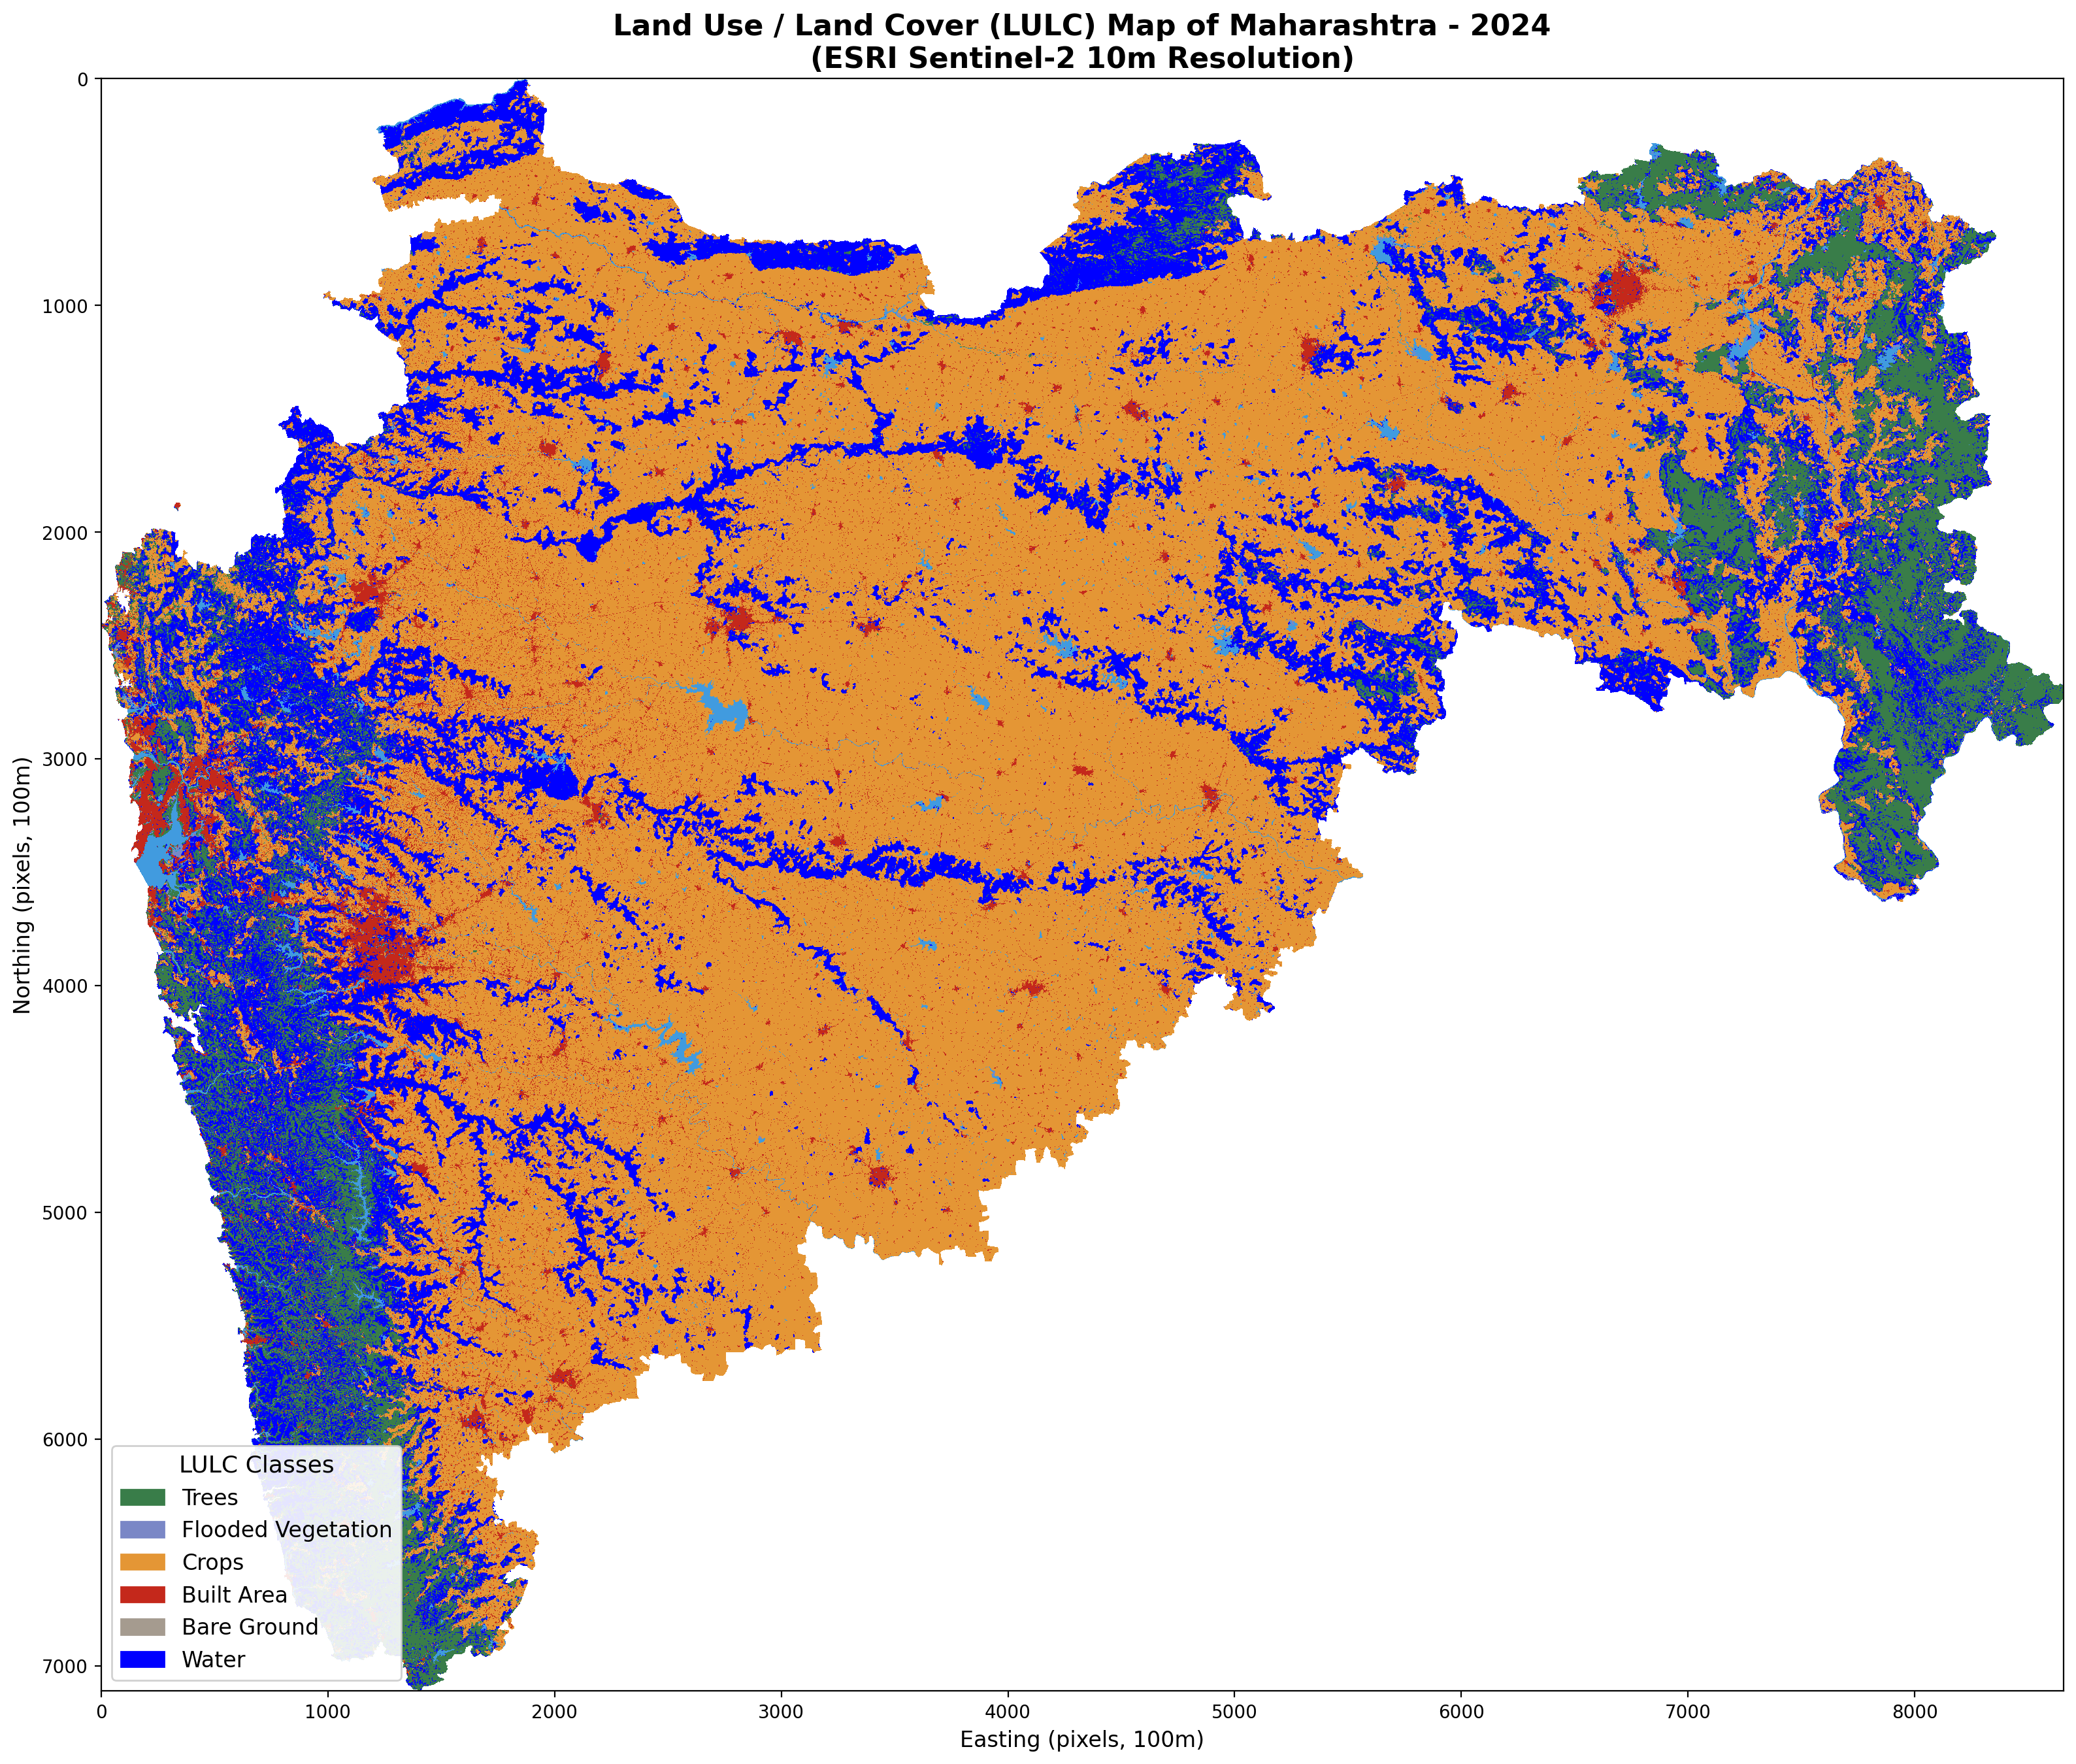
\includegraphics[width=0.6\textwidth]{fig1_maharashtra_lulc_map_2024.png}
\caption{Land Use / Land Cover map of Maharashtra for 2024 derived from ESRI Sentinel-2 10m data. Crops (orange) dominate the central and eastern Deccan Plateau, while Trees (green) are concentrated along the Western Ghats. Built Area (red) clusters are visible around Mumbai--Pune and other urban centers.}
\label{fig:lulc_map}
\end{figure}

\begin{figure}[H]
\centering
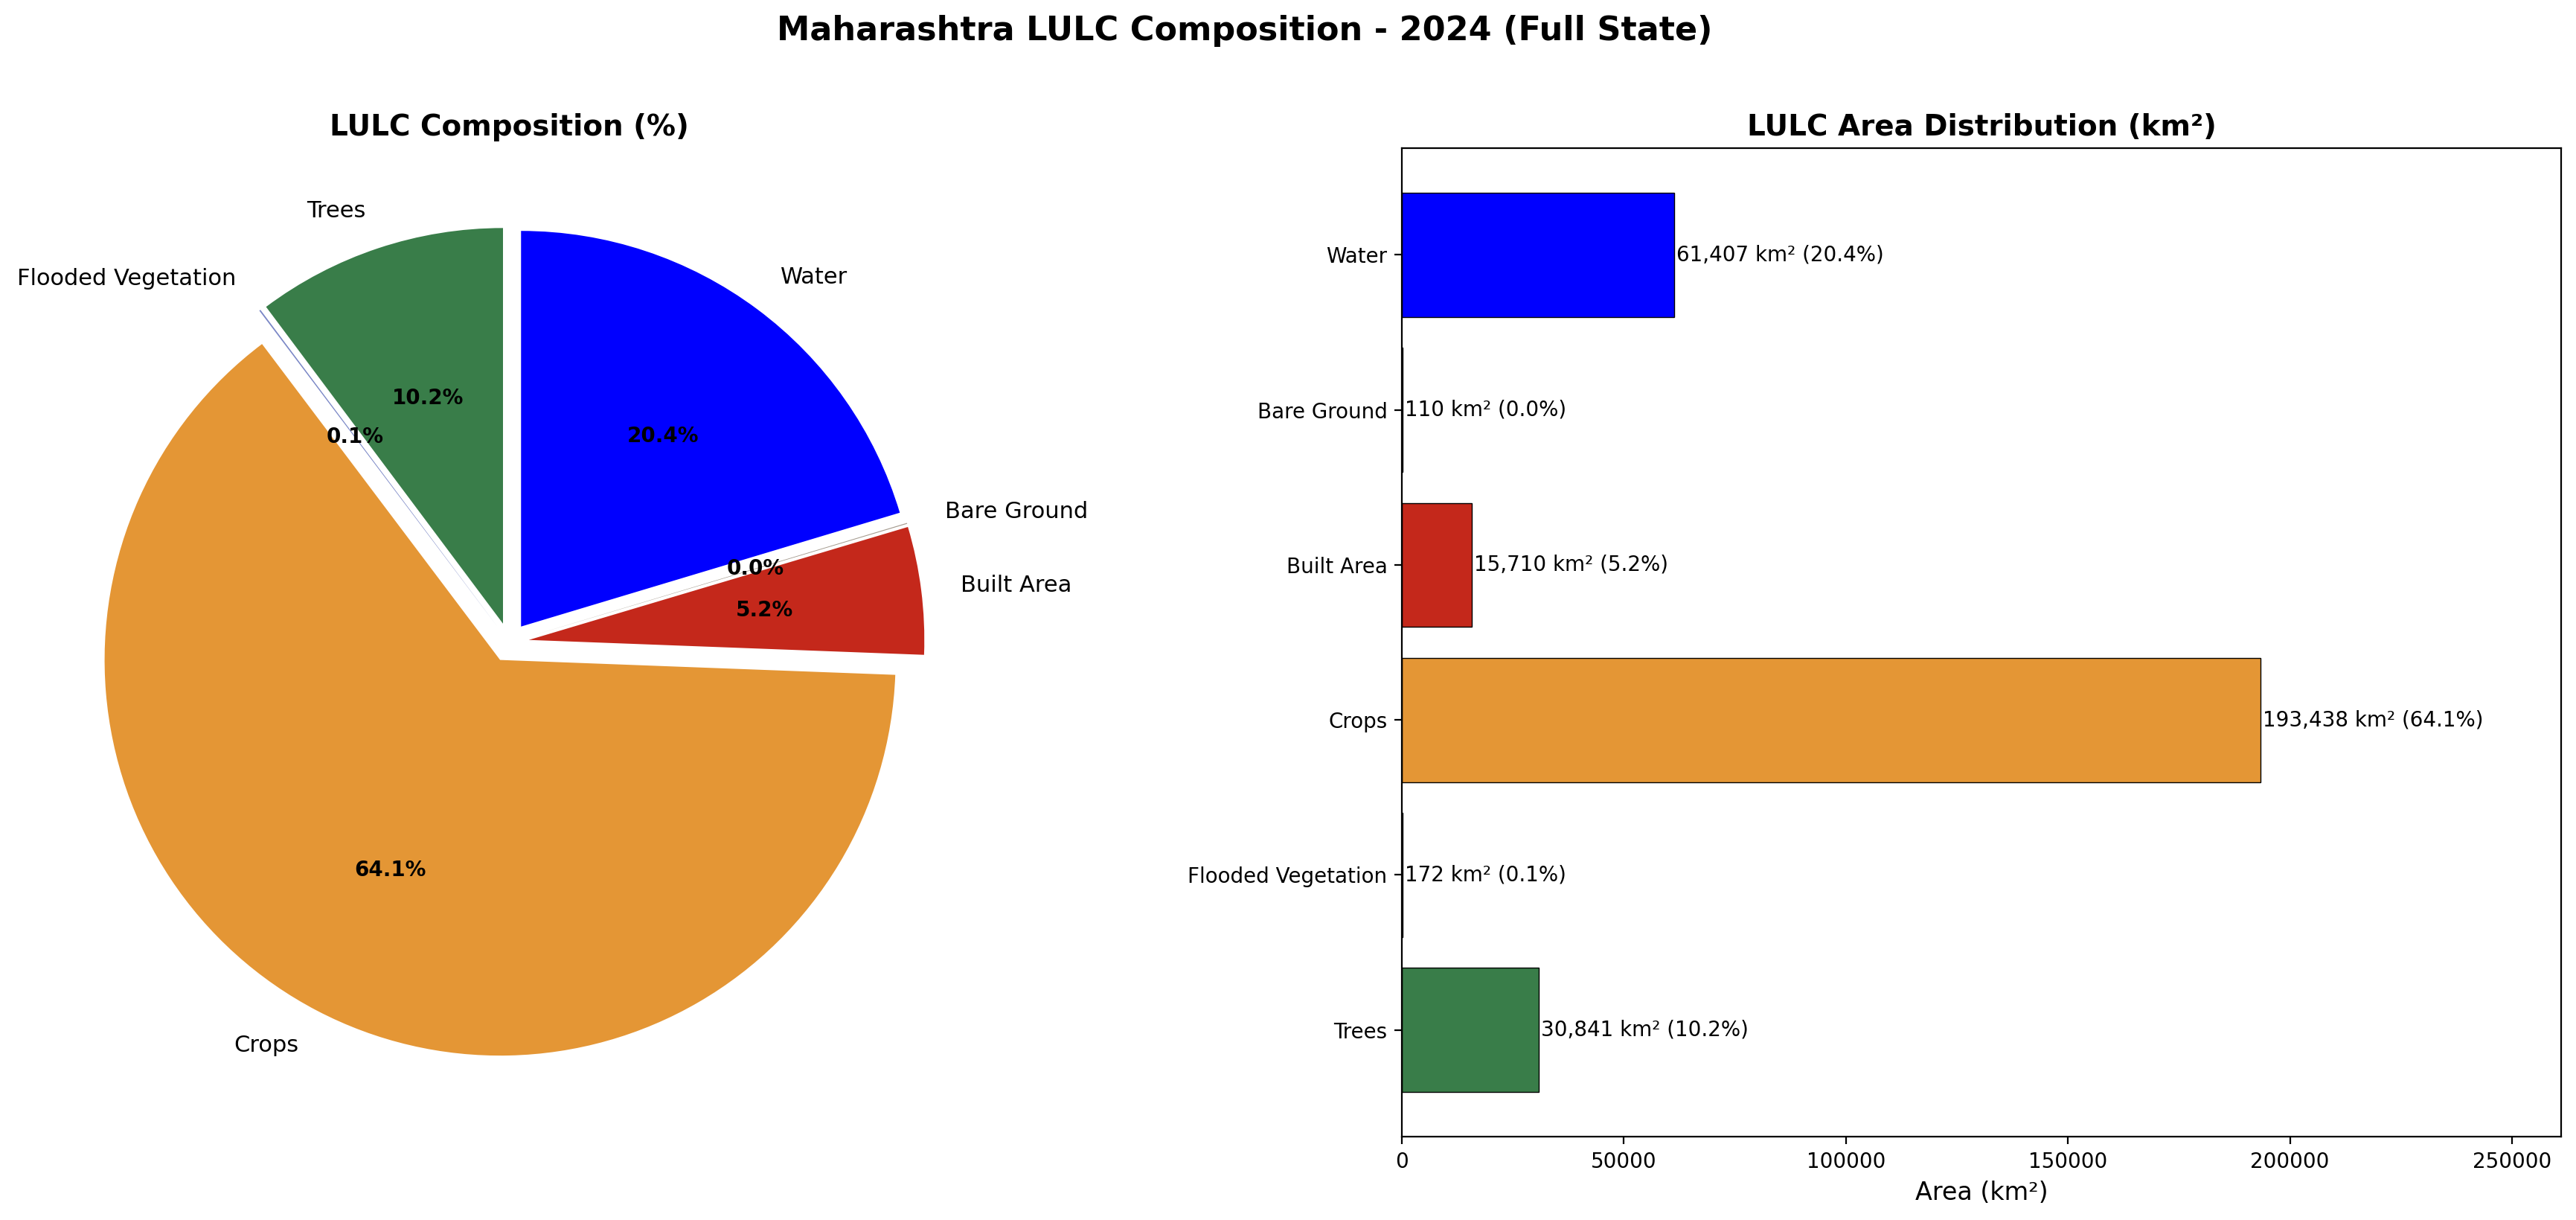
\includegraphics[width=0.9\textwidth]{fig2_lulc_composition_2024.png}
\caption{LULC composition of Maharashtra (2024): percentage distribution (left) and absolute area in km\textsuperscript{2} (right).}
\label{fig:composition}
\end{figure}

The analysis reveals that \textbf{Crops} (193,438~km\textsuperscript{2}, 64.1\%) dominate, followed by \textbf{Water} (61,407~km\textsuperscript{2}, 20.4\%, including coastal areas), \textbf{Trees} (30,841~km\textsuperscript{2}, 10.2\%, concentrated in the Western Ghats and eastern Vidarbha forests), and \textbf{Built Area} (15,710~km\textsuperscript{2}, 5.2\%, centered around Mumbai, Pune, Nashik, and Nagpur). The total classified area of $\sim$301,679~km\textsuperscript{2} closely matches Maharashtra's official area of $\sim$307,713~km\textsuperscript{2}.

\subsection{District-Level LULC Distribution (2024)}

Figure~\ref{fig:choropleth} presents choropleth maps of the four major LULC classes at the district level.

\begin{figure}[H]
\centering
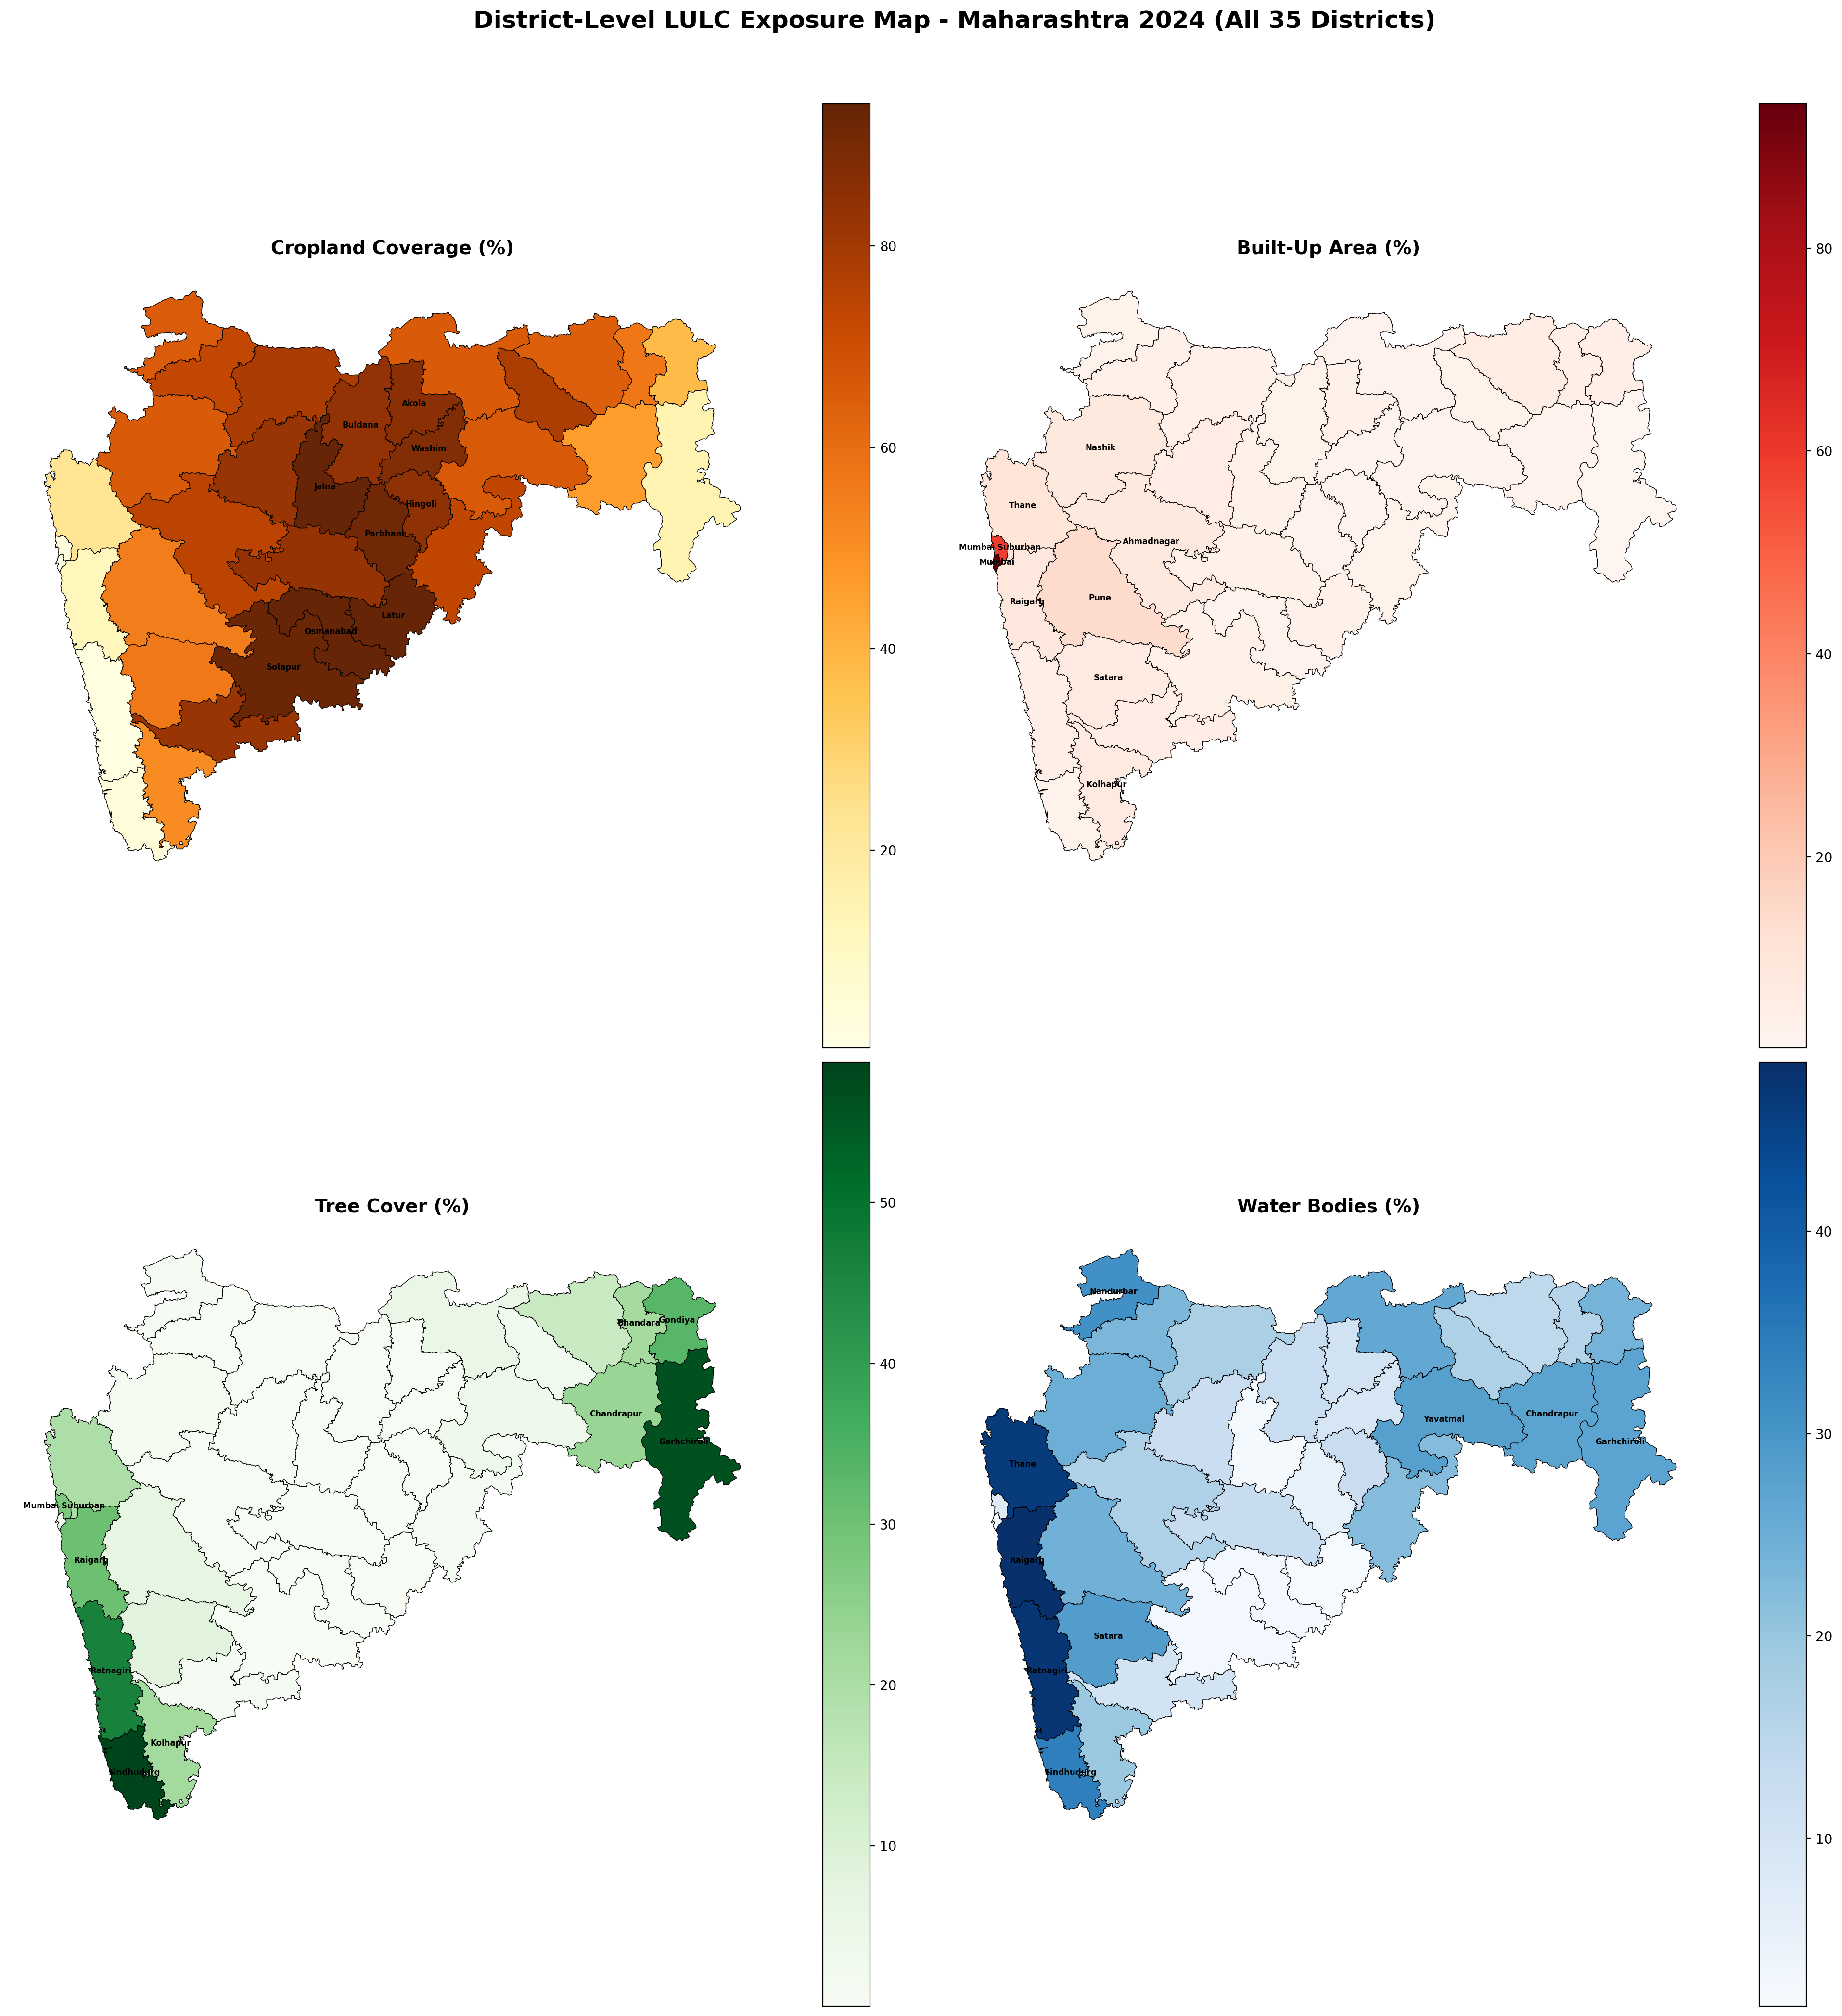
\includegraphics[width=0.9\textwidth]{fig3_district_choropleth_2024.png}
\caption{District-level LULC exposure maps for Maharashtra (2024). Top-left: Cropland; Top-right: Built-up; Bottom-left: Tree cover; Bottom-right: Water.}
\label{fig:choropleth}
\end{figure}

Key observations: \textbf{Highest cropland}---Osmanabad (94.1\%), Jalna (94.0\%), Latur (93.7\%), all in drought-prone Marathwada. \textbf{Highest built-up}---Mumbai (94.2\%), Mumbai Suburban (58.9\%), Pune (14.0\%). \textbf{Highest tree cover}---Sindhudurg (58.7\%), Garhchiroli (56.6\%), Ratnagiri (46.1\%), spanning the Western Ghats and eastern Vidarbha. \textbf{Highest water}---Raigarh (48.4\%), Ratnagiri (47.4\%), Thane (46.3\%)---coastal districts with estuarine influence.

\subsection{Temporal Change Detection: 2017 vs.\ 2024}

Figure~\ref{fig:change} shows the percentage point change in each LULC class at the district level, and Figure~\ref{fig:temporal} provides the state-level comparison.

\begin{figure}[H]
\centering
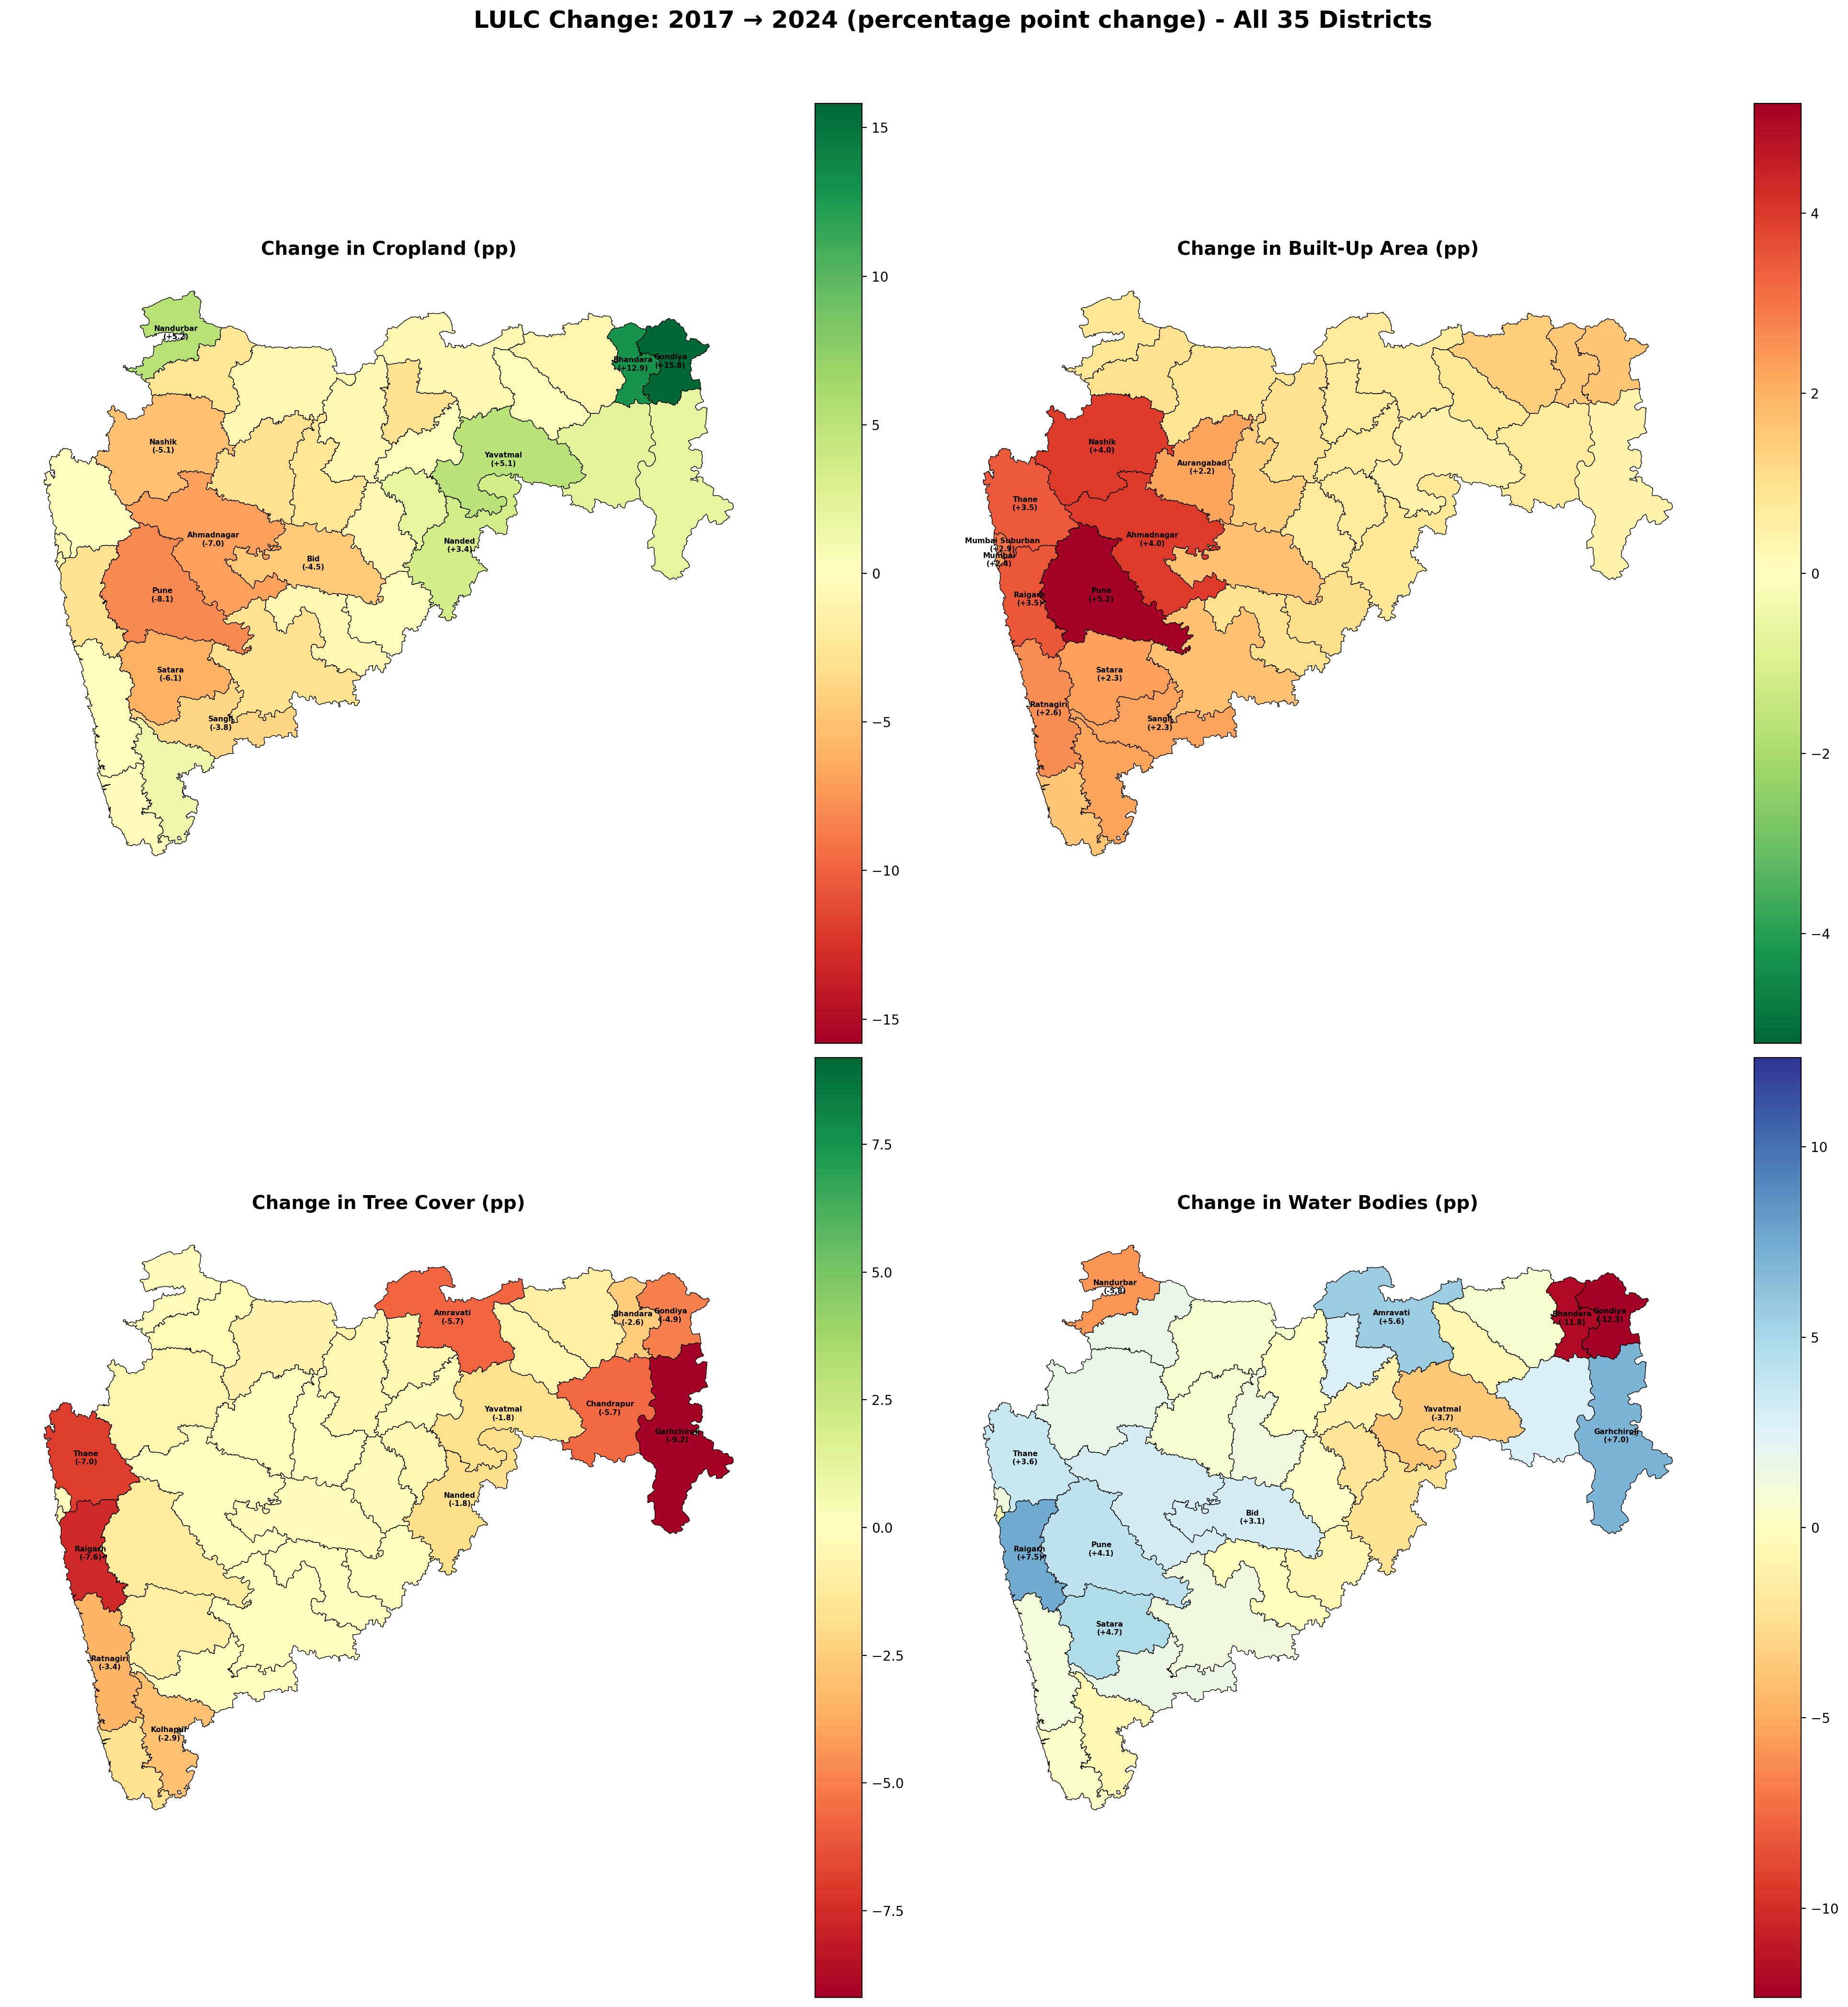
\includegraphics[width=0.9\textwidth]{fig4_change_detection_2017_2024.png}
\caption{District-level LULC change from 2017 to 2024 expressed as percentage point (pp) change. Red indicates loss; green indicates gain.}
\label{fig:change}
\end{figure}

\begin{figure}[H]
\centering
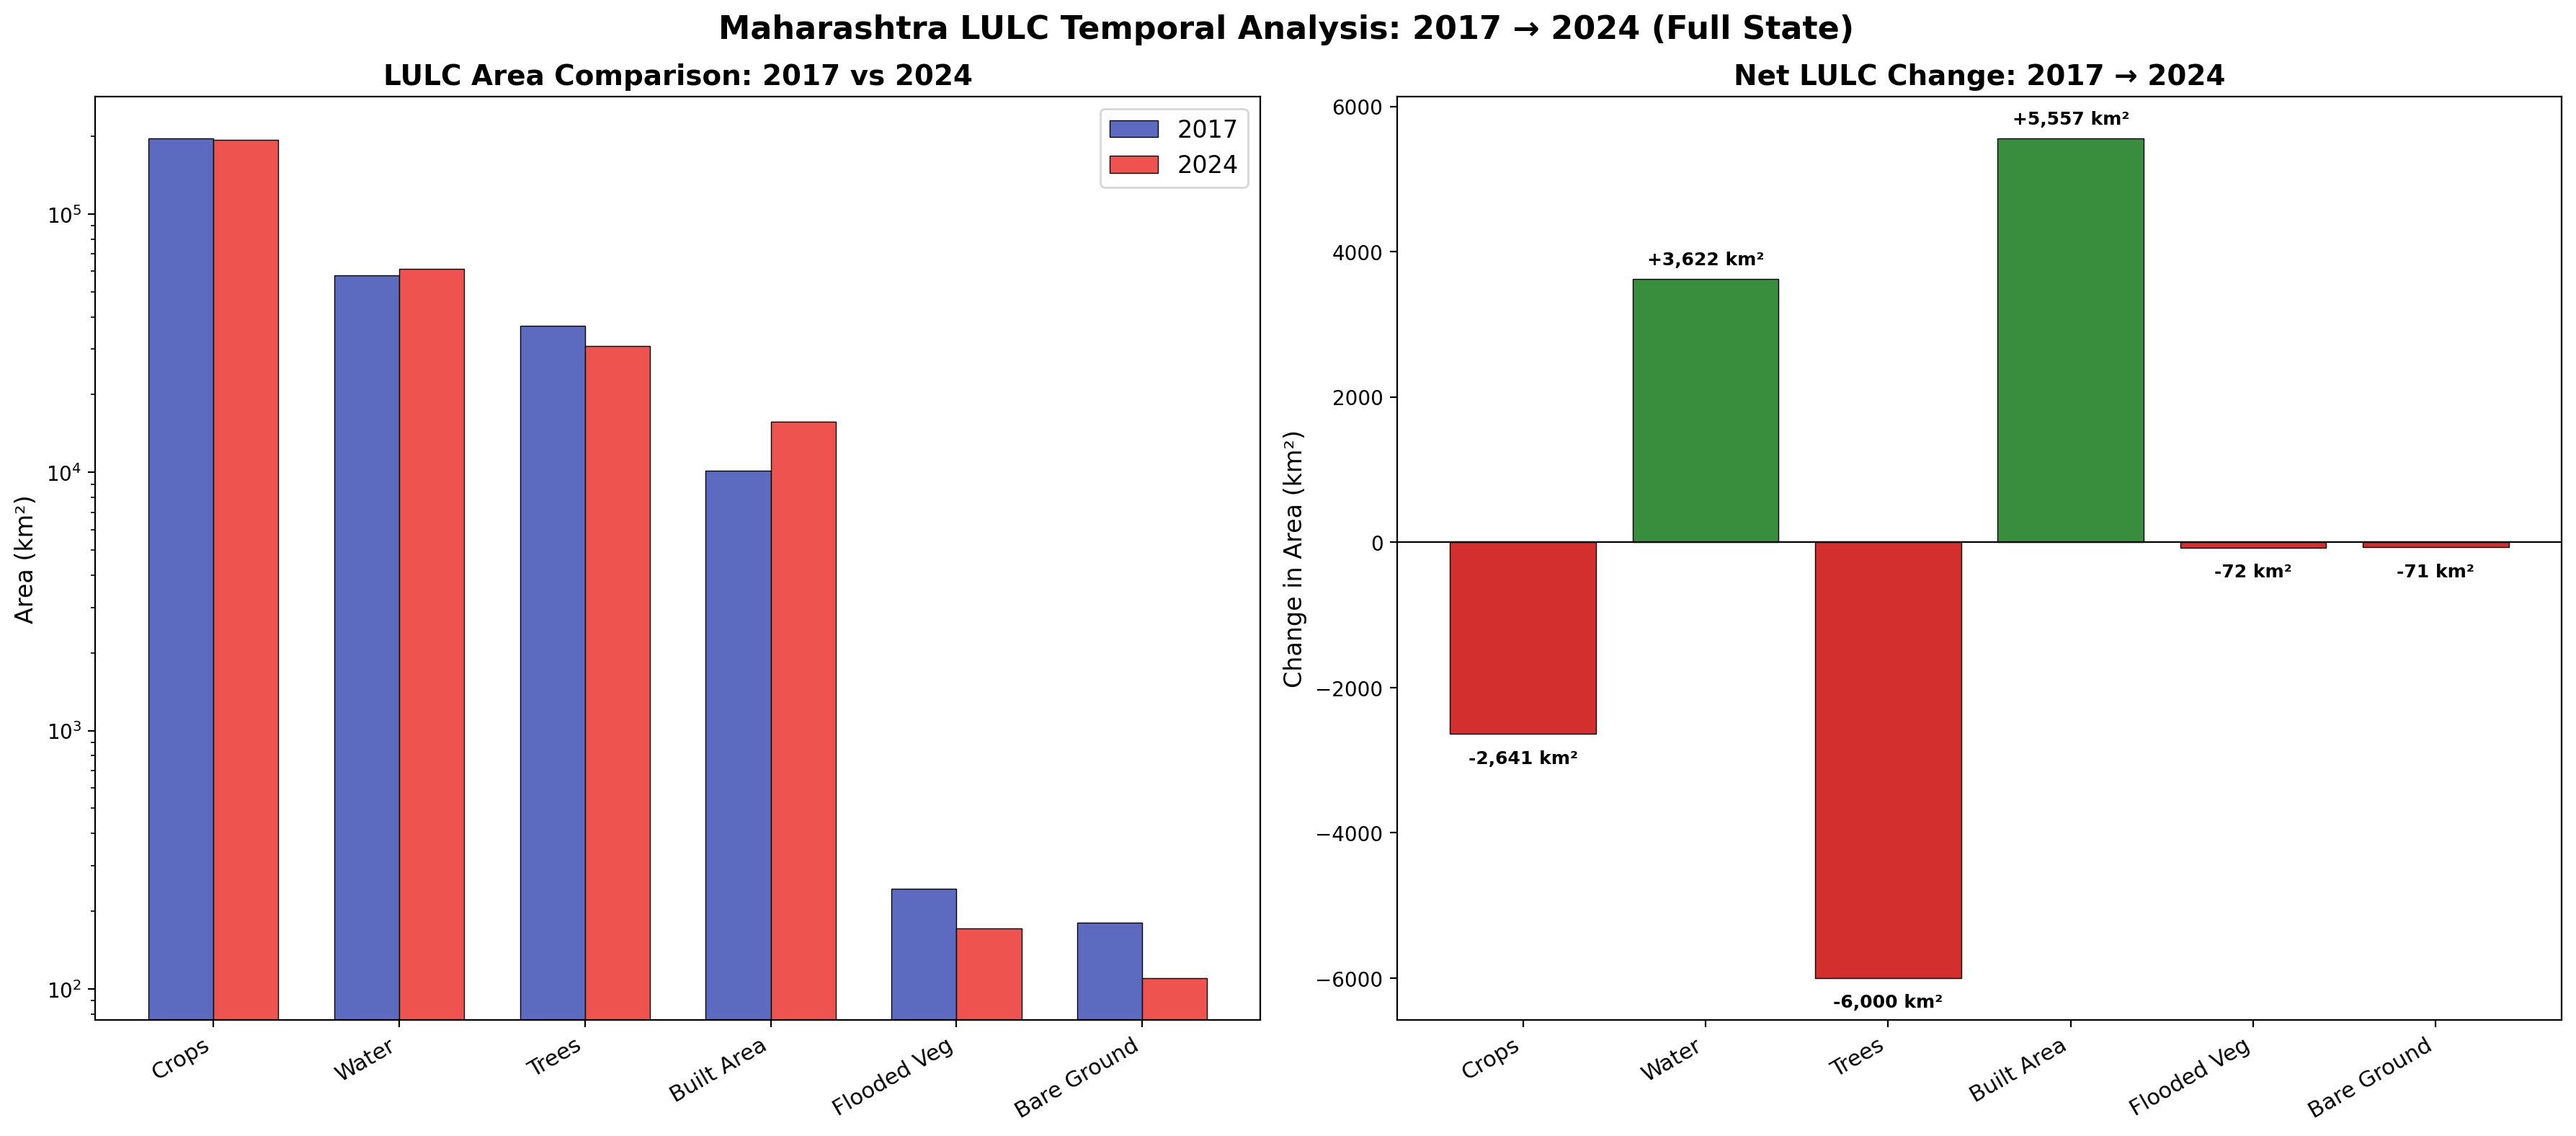
\includegraphics[width=0.9\textwidth]{fig8_temporal_comparison.png}
\caption{State-level LULC comparison between 2017 and 2024: absolute area (left, log scale) and net change in km\textsuperscript{2} (right).}
\label{fig:temporal}
\end{figure}

The temporal analysis reveals three major trends at the state level over the 7-year period:

\begin{enumerate}
    \item \textbf{Rapid urbanization:} Built-up area increased by \textbf{+5,557~km\textsuperscript{2}} (+54.7\%), from 10,153~km\textsuperscript{2} in 2017 to 15,710~km\textsuperscript{2} in 2024. This represents a rate of $\sim$794~km\textsuperscript{2}/year of new built-up land. Pune, Ahmadnagar, and Nashik are the top urbanizing districts.

    \item \textbf{Deforestation:} Tree cover declined by \textbf{--6,000~km\textsuperscript{2}} (--16.3\%), from 36,841~km\textsuperscript{2} to 30,841~km\textsuperscript{2}. The most affected districts include those in the ecologically sensitive Western Ghats-Konkan region (Thane, Raigarh, Ratnagiri) as well as eastern Vidarbha (Garhchiroli lost $\sim$9 percentage points of tree cover).

    \item \textbf{Cropland contraction:} Agricultural land decreased by \textbf{--2,641~km\textsuperscript{2}} (--1.3\%), from 196,079~km\textsuperscript{2} to 193,438~km\textsuperscript{2}. Pune and Nashik lost the most cropland, largely to urban expansion.
\end{enumerate}

Figure~\ref{fig:top_changers} highlights the districts with the largest absolute changes.

\begin{figure}[H]
\centering
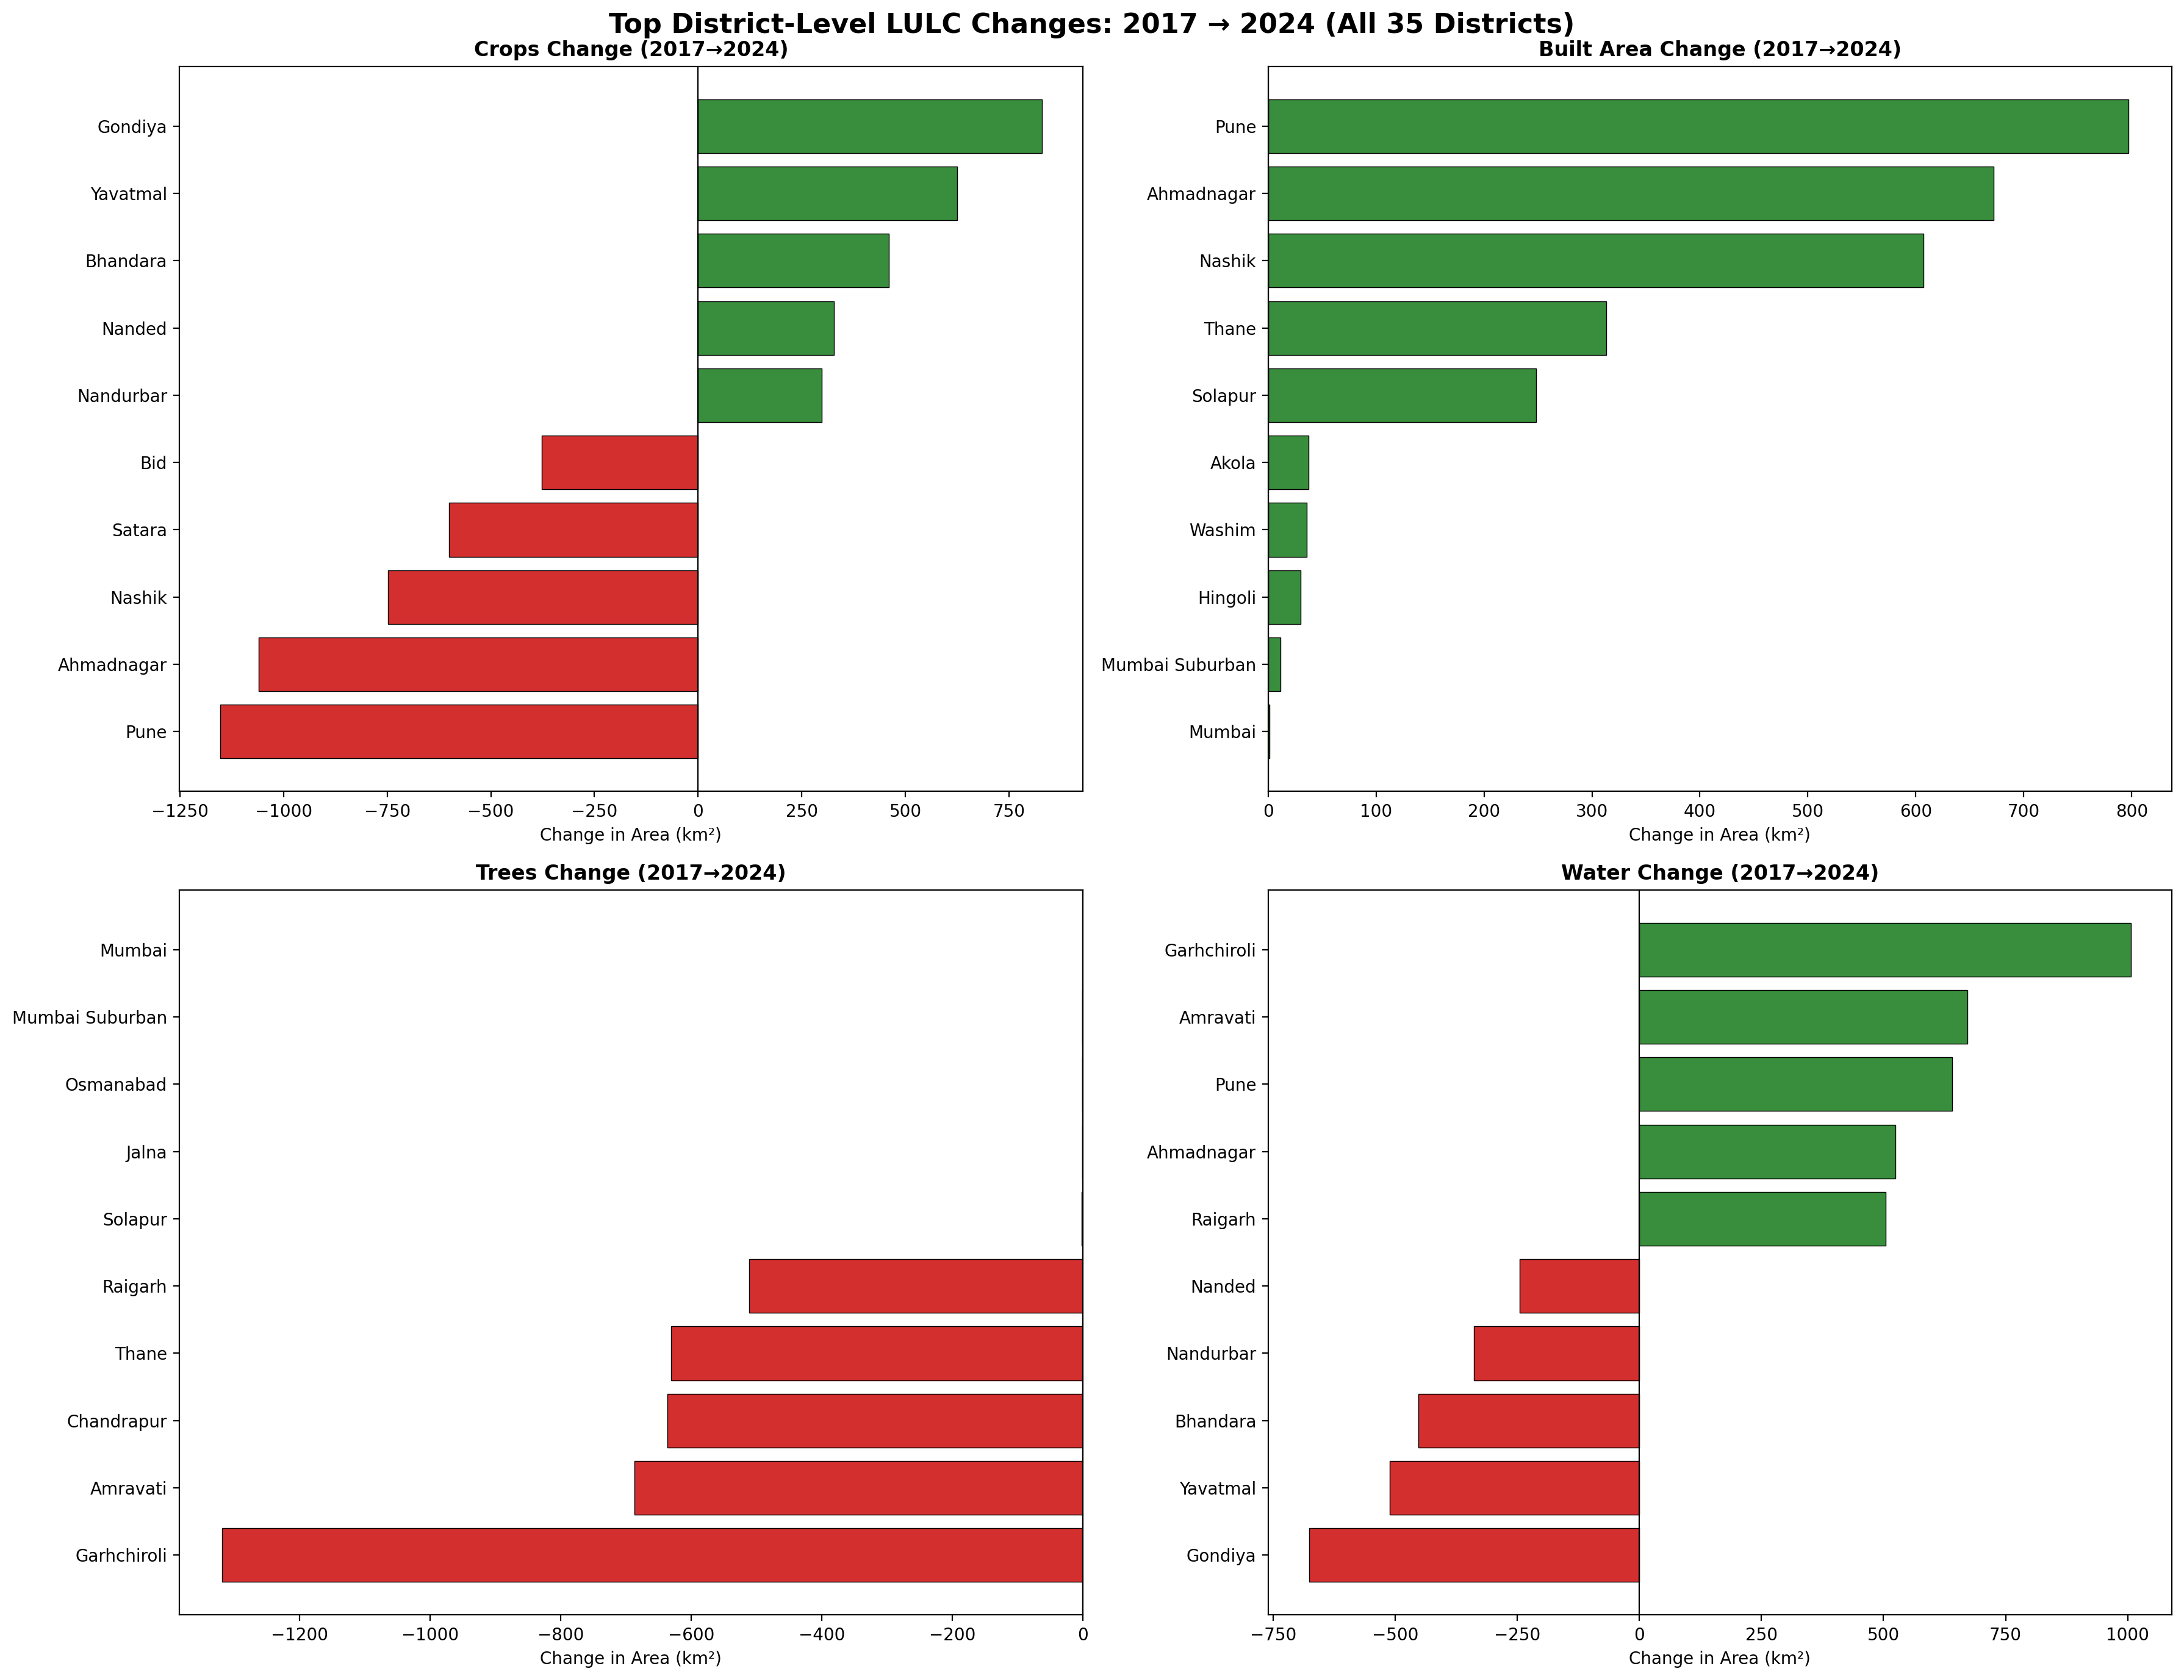
\includegraphics[width=0.9\textwidth]{fig5_top_changers_2017_2024.png}
\caption{Top 5 gaining and losing districts for each LULC class (2017--2024) by absolute area change (km\textsuperscript{2}).}
\label{fig:top_changers}
\end{figure}

\subsection{Gridded Spatial Analysis}

Figure~\ref{fig:gridded} presents the 25~km $\times$ 25~km gridded heatmaps, providing a spatially continuous view of LULC intensity unbiased by administrative boundary shapes.

\begin{figure}[H]
\centering
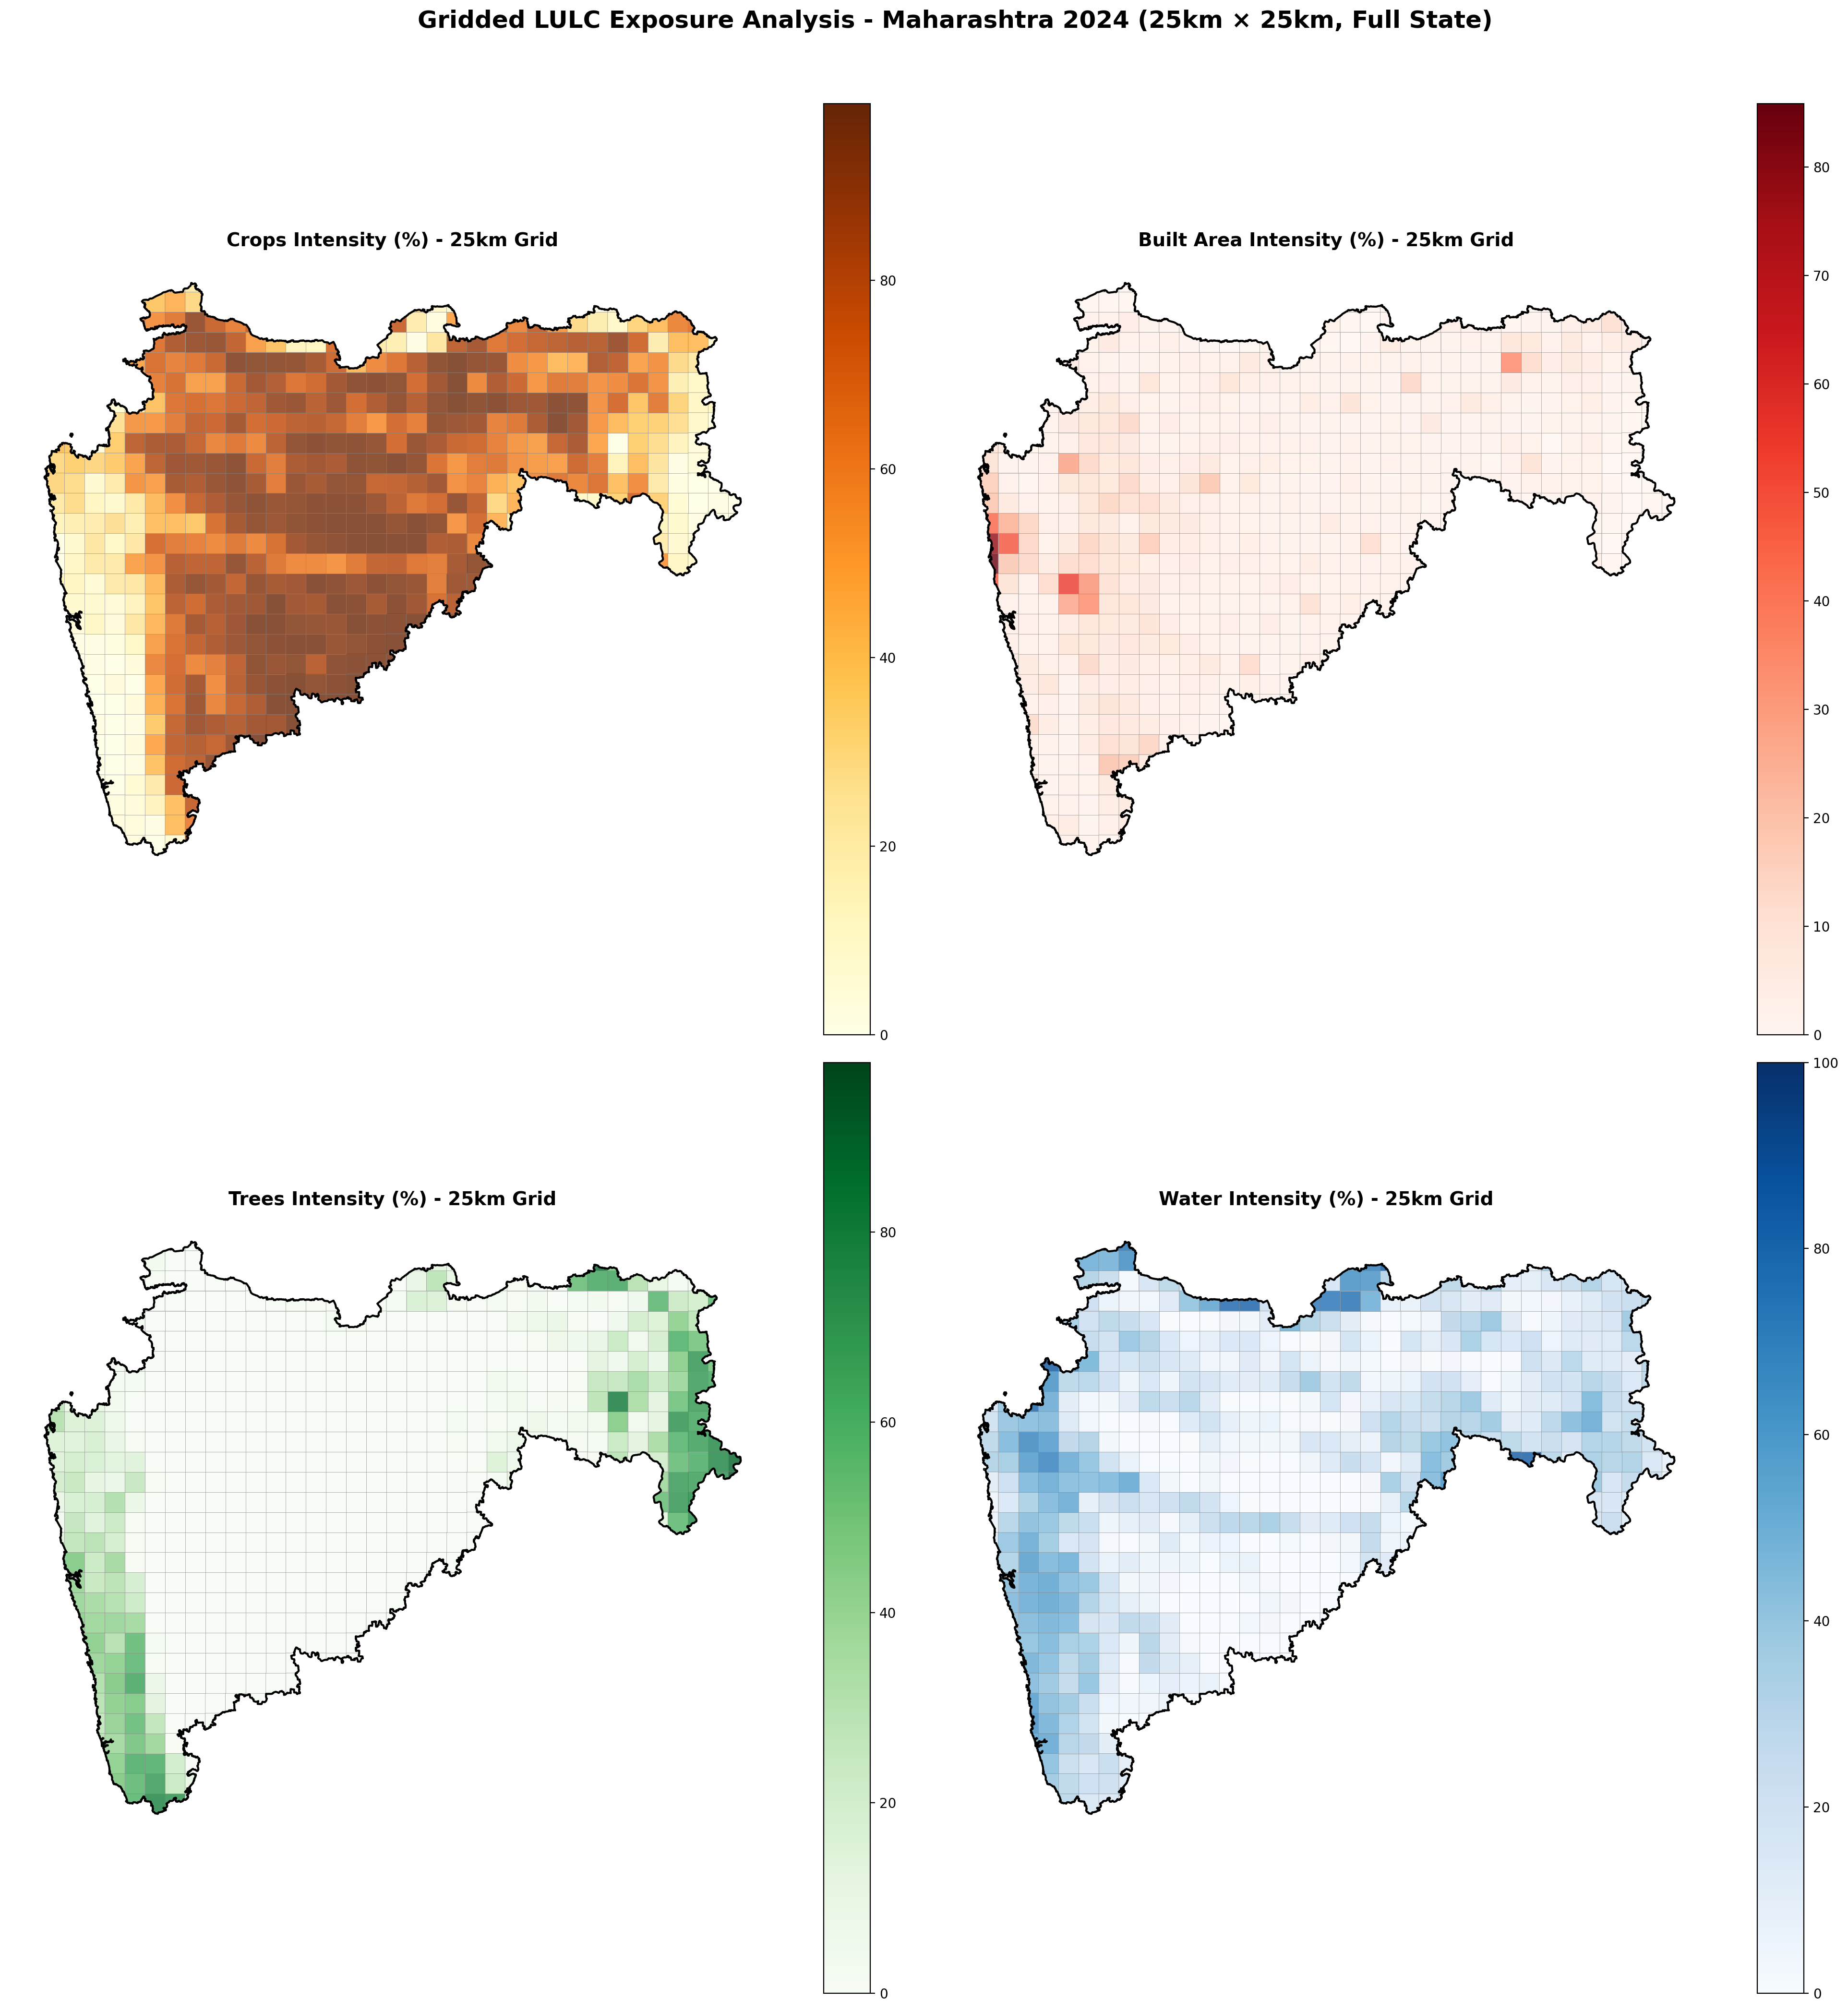
\includegraphics[width=0.9\textwidth]{fig6_gridded_heatmap_2024.png}
\caption{Gridded (25~km $\times$ 25~km) LULC intensity heatmaps for Maharashtra (2024). The gridded view reveals spatial gradients not visible in district-level choropleth maps.}
\label{fig:gridded}
\end{figure}

The gridded analysis reveals a strong east-west crop intensity gradient (near-100\% on the Deccan Plateau), tightly concentrated built-up hotspots around Mumbai--Pune, tree cover confined to the Western Ghats and eastern Vidarbha, and increasing water intensity toward the coast.

\subsection{Climate Risk Exposure Index}

Figure~\ref{fig:risk} presents the composite Climate Risk Exposure Index (CREI) and its component sub-indicators.

\begin{figure}[H]
\centering
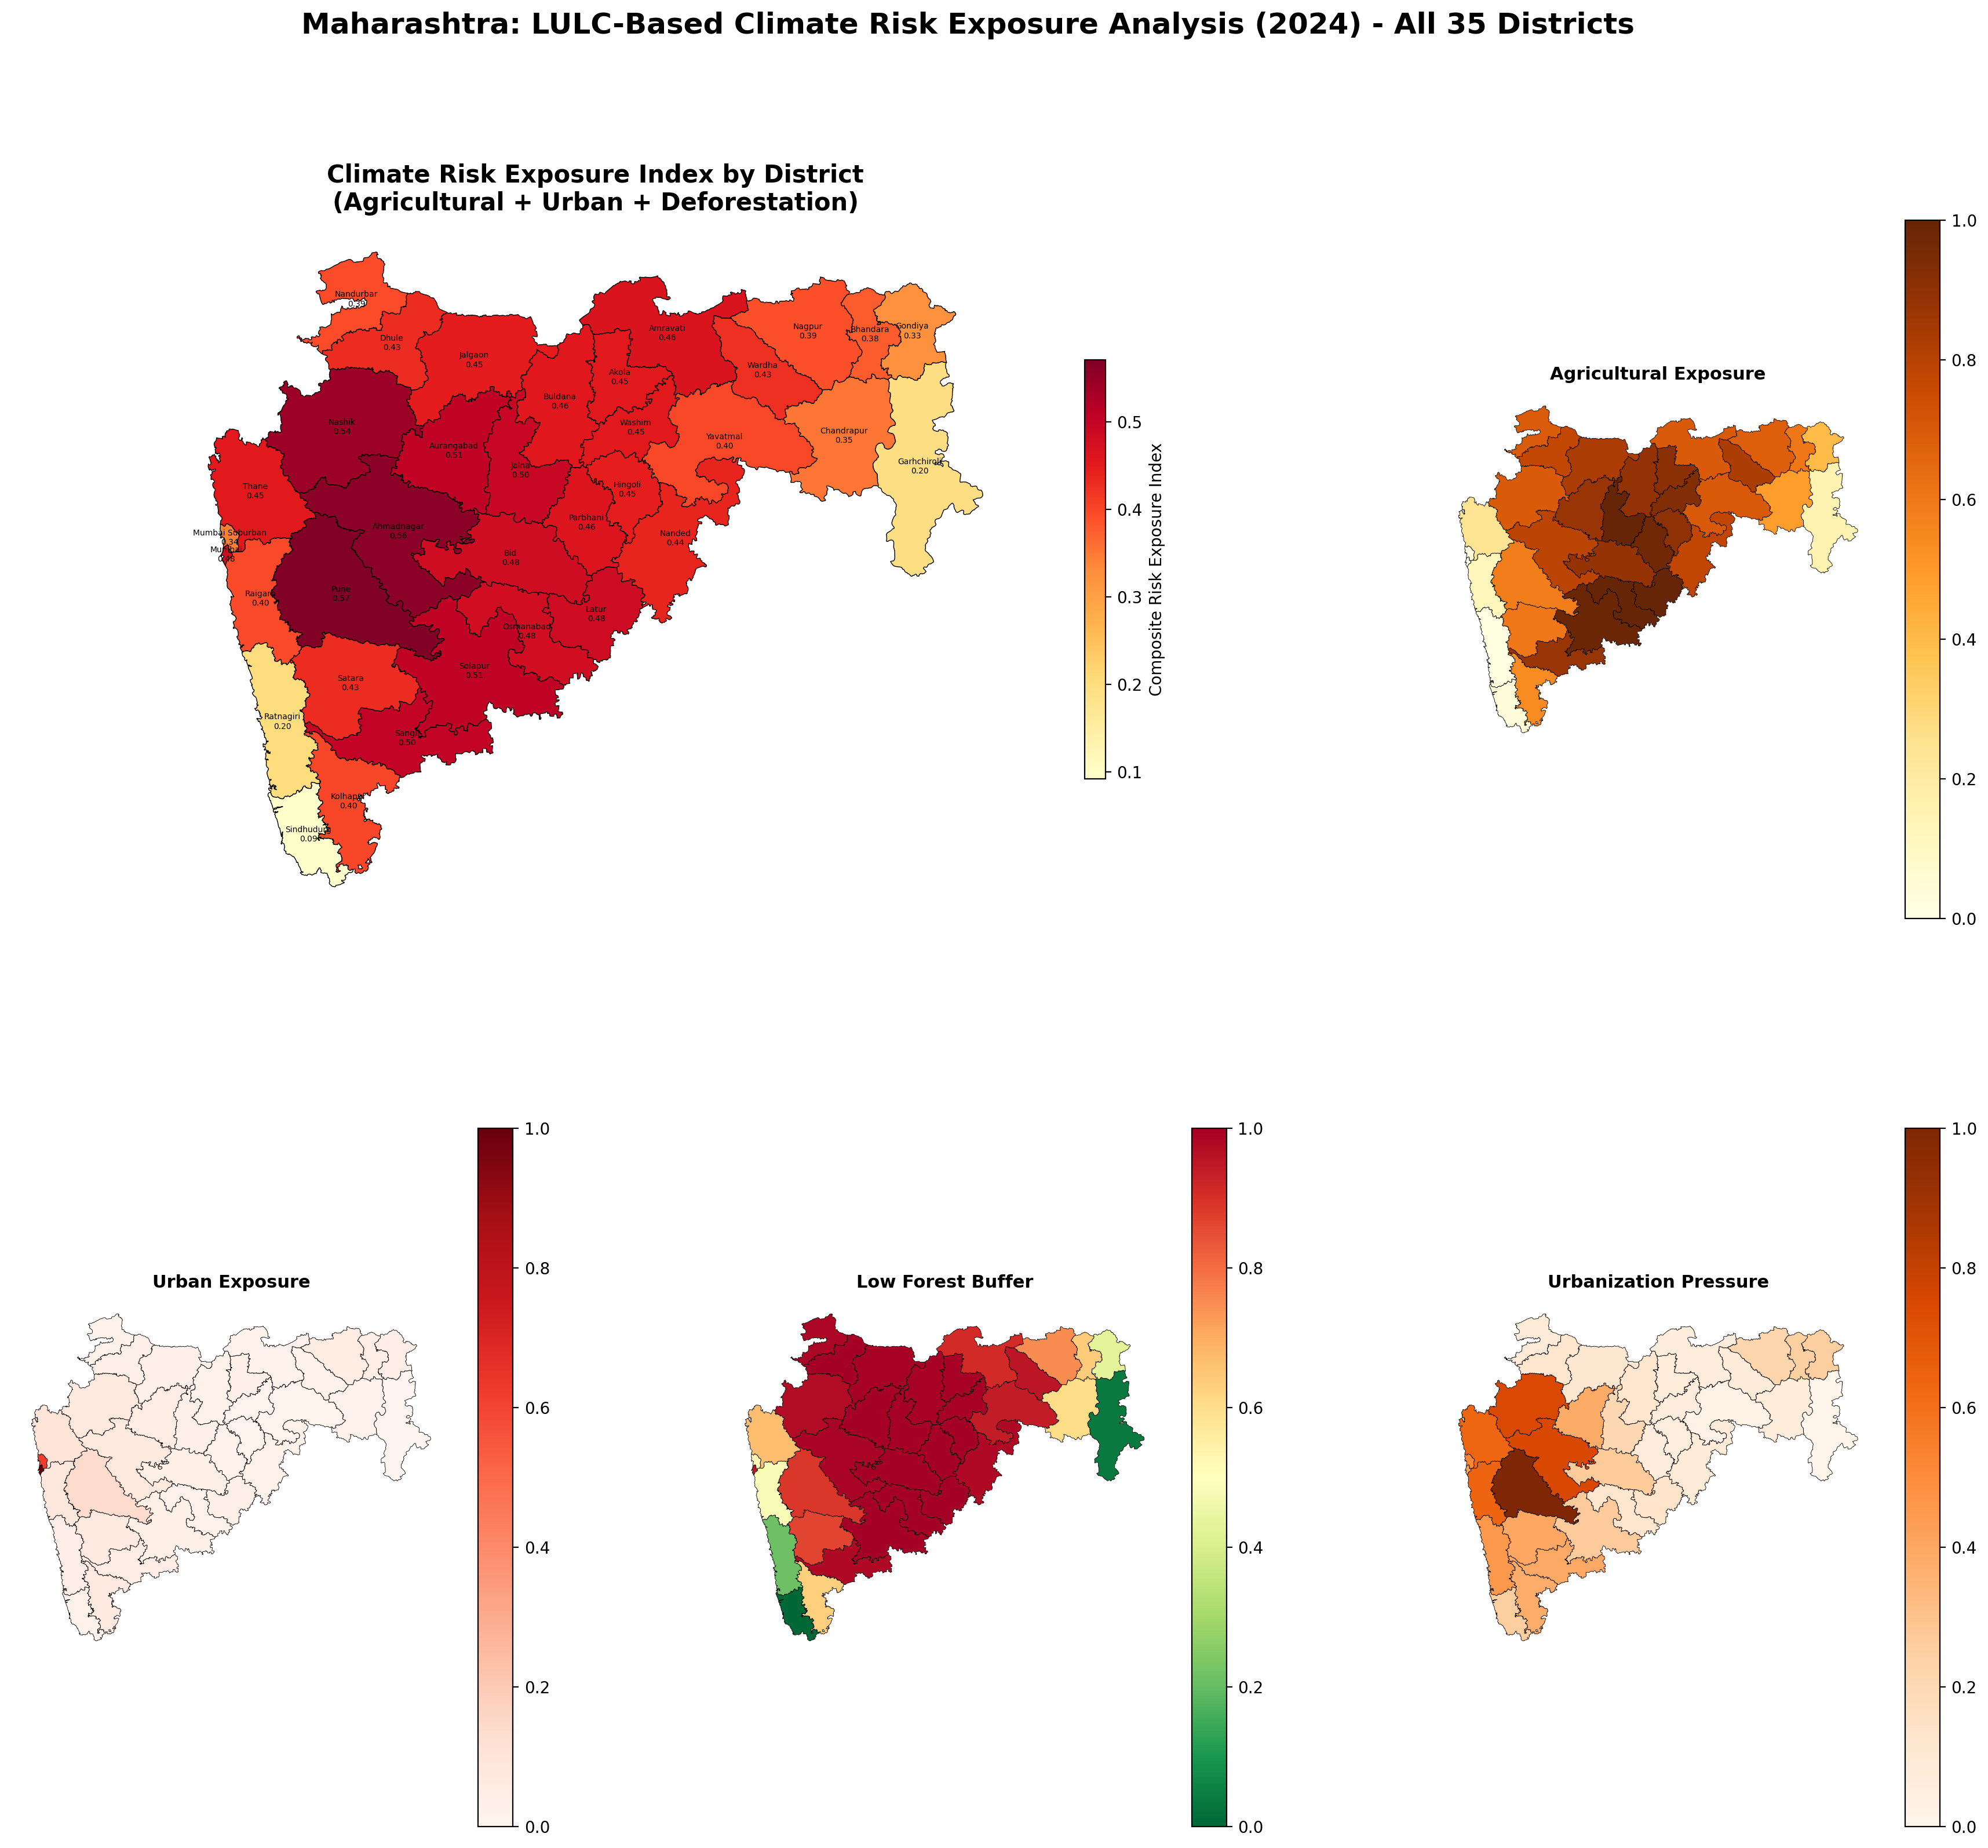
\includegraphics[width=0.9\textwidth]{fig7_climate_risk_exposure.png}
\caption{LULC-based Climate Risk Exposure Index for Maharashtra (2024). The main map shows the composite index; sub-maps show individual components: Agricultural Exposure, Urban Exposure, Low Forest Buffer, and Urbanization Pressure.}
\label{fig:risk}
\end{figure}

Table~\ref{tab:risk_top10} lists the 10 most exposed districts.

\begin{table}[H]
\centering
\caption{Top 10 most climate-exposed districts in Maharashtra ranked by CREI.}
\label{tab:risk_top10}
\begin{tabular}{clccccc}
\toprule
\textbf{Rank} & \textbf{District} & \textbf{CREI} & \textbf{$E_{agri}$} & \textbf{$E_{urban}$} & \textbf{$E_{forest}$} & \textbf{$E_{urb\_press}$} \\
\midrule
1  & Pune        & 0.571 & 0.59 & 0.15 & 0.89 & 1.00 \\
2  & Ahmadnagar  & 0.560 & 0.79 & 0.08 & 0.99 & 0.80 \\
3  & Nashik      & 0.542 & 0.70 & 0.08 & 0.97 & 0.72 \\
4  & Solapur     & 0.507 & 0.99 & 0.04 & 1.00 & 0.27 \\
5  & Aurangabad  & 0.506 & 0.87 & 0.06 & 1.00 & 0.40 \\
6  & Sangli      & 0.503 & 0.87 & 0.06 & 0.98 & 0.33 \\
7  & Jalna       & 0.496 & 1.00 & 0.04 & 1.00 & 0.18 \\
8  & Latur       & 0.485 & 1.00 & 0.04 & 1.00 & 0.10 \\
9  & Bid         & 0.483 & 0.88 & 0.04 & 1.00 & 0.20 \\
10 & Mumbai      & 0.479 & 0.00 & 1.00 & 0.98 & 0.02 \\
\bottomrule
\end{tabular}
\end{table}

The CREI reveals two exposure archetypes: (1)~\textbf{Pune, Ahmadnagar, Nashik} (CREI 0.54--0.57)---peri-urban transition zones with combined agricultural, urbanization, and low-forest pressures; and (2)~\textbf{Solapur, Jalna, Latur, Bid} (CREI 0.48--0.51)---Marathwada districts with extreme crop dependence and zero forest buffer. The \textbf{least exposed}---Sindhudurg (0.092), Garhchiroli (0.195), Ratnagiri (0.201)---benefit from dense forest cover providing natural climate resilience.

% ══════════════════════════════════════════════════════════════
\section{Applications of LULC Analysis}
% ══════════════════════════════════════════════════════════════

The LULC exposure mapping and the derived Climate Risk Exposure Index presented in this study have a wide range of practical applications across multiple domains:

\begin{enumerate}
    \item \textbf{Disaster Risk Reduction and Early Warning Systems.} District-level LULC data can be integrated into flood and drought early warning frameworks. Districts with high cropland percentages and negligible forest buffer (e.g., Osmanabad, Jalna) can be flagged for priority drought monitoring, while rapidly urbanizing districts (e.g., Pune, Thane) can be targeted for flash flood risk assessments based on increasing impervious surface coverage \citep{ipcc2022}.

    \item \textbf{Urban and Regional Planning.} The spatial mapping of built-up area expansion provides planners with evidence-based inputs for zoning regulations, green infrastructure allocation, and smart city initiatives. The 25~km gridded analysis is particularly suited for identifying peri-urban transition zones where development controls are most needed, and for planning buffer green belts around expanding urban cores.

    \item \textbf{Agricultural Insurance and Crop Management.} Insurance agencies and agricultural departments can use the district-wise cropland exposure data to design index-based crop insurance products. The temporal change data (2017--2024) helps identify districts where agricultural land is being lost to urbanization, enabling proactive land-use policy interventions and targeted subsidies for climate-resilient farming practices \citep{mall2006water}.

    \item \textbf{Forest Conservation and Biodiversity Protection.} The identification of two distinct deforestation fronts---the Western Ghats-Konkan belt and the eastern Vidarbha corridor---directly supports conservation prioritization. These findings can inform REDD+ (Reducing Emissions from Deforestation and Forest Degradation) strategies, wildlife corridor planning, and Environmental Impact Assessment (EIA) screenings for proposed development projects in ecologically sensitive zones \citep{myers2000biodiversity}.

    \item \textbf{Climate Adaptation Planning and Policy.} The composite CREI provides a single, interpretable metric that policymakers can use to allocate climate adaptation funds across districts. High-CREI districts can be prioritized for interventions such as watershed management programs, urban heat island mitigation infrastructure (cool roofs, urban forestry), and community-based adaptation projects under the National Action Plan on Climate Change (NAPCC).

    \item \textbf{Carbon Accounting and Net-Zero Targets.} Tree cover extent and change data are essential inputs for estimating terrestrial carbon stocks and fluxes. The 6,000~km\textsuperscript{2} loss in tree cover identified in this study implies a significant reduction in carbon sequestration capacity, which is directly relevant to Maharashtra's contributions to India's Nationally Determined Contributions (NDCs) under the Paris Agreement \citep{bonan2008forests}.

    \item \textbf{Water Resource Management.} LULC composition strongly influences watershed hydrology---forested catchments retain water and reduce peak flows, while urbanized catchments generate higher runoff. The district-level and gridded LULC data can be coupled with hydrological models (e.g., SWAT, HEC-HMS) to improve reservoir operation, irrigation planning, and groundwater recharge zone identification across Maharashtra's river basins.
\end{enumerate}

% ══════════════════════════════════════════════════════════════
\section{Conclusions and Discussion}
% ══════════════════════════════════════════════════════════════

This study presents a comprehensive spatial analysis of LULC exposure in Maharashtra using high-resolution (10m) Sentinel-2 land cover data at state, district, and gridded (25~km) scales. The major conclusions are:

\begin{enumerate}
    \item \textbf{Agricultural dominance and drought exposure.} Maharashtra is overwhelmingly agrarian (64.1\% cropland). The Marathwada plateau shows near-total crop dependence ($>$90\% in Osmanabad, Jalna, Latur), with zero forest buffer, making these districts acutely vulnerable to drought and monsoon variability \citep{gadgil2003indian}.

    \item \textbf{Rapid urbanization.} Built-up area increased by 54.7\% (+5,557~km\textsuperscript{2}) between 2017 and 2024---a rate of $\sim$794~km\textsuperscript{2}/year. This sprawl exacerbates urban heat island effects and reduces natural drainage capacity \citep{oke1982energetic}. The Pune--Nashik--Ahmadnagar corridor is the primary epicenter.

    \item \textbf{Deforestation across two forest belts.} Tree cover declined by 16.3\% (--6,000~km\textsuperscript{2}), affecting both the Western Ghats-Konkan region (a UNESCO biodiversity hotspot) and the eastern Vidarbha forests (Garhchiroli, Gondiya), which form a contiguous Central Indian corridor critical for tiger habitat \citep{myers2000biodiversity}.

    \item \textbf{Spatial gradients revealed by gridded analysis.} The 25~km grid analysis exposes a crop-dominated interior plateau, two distinct forest belts, and tightly concentrated urban hotspots---patterns masked in coarser administrative analyses.

    \item \textbf{Risk ranking.} The CREI identifies Pune, Ahmadnagar, and Nashik as the most exposed districts (compound effect of agricultural dependence, rapid urbanization, negligible forest buffer). Sindhudurg, Garhchiroli, and Ratnagiri are least exposed, protected by dense forest cover.

    \item \textbf{Policy implications.} These findings support targeted strategies: drought-resilient agriculture in Marathwada, urban heat mitigation in the Pune--Mumbai corridor, and forest conservation in the Western Ghats and Garhchiroli--Gondiya belt.
\end{enumerate}

\textbf{Limitations.} (1)~The ESRI LULC product has $\sim$85\% global accuracy with potential local misclassifications; (2)~the water percentage (20.4\%) includes coastal ocean areas; (3)~CREI weights are judgment-based and could be refined via multi-criteria decision analysis; (4)~reprojection of tile 44Q from UTM Zone 44N to 43N may introduce minor distortions.

% ══════════════════════════════════════════════════════════════
% References
% ══════════════════════════════════════════════════════════════
\newpage
\bibliographystyle{apalike}

\begin{thebibliography}{99}

\bibitem[Bonan, 2008]{bonan2008forests}
Bonan, G. B. (2008).
\newblock Forests and climate change: Forcings, feedbacks, and the climate benefits of forests.
\newblock \textit{Science}, 320(5882), 1444--1449.
\newblock \url{https://doi.org/10.1126/science.1155121}

\bibitem[DataMeet, 2023]{datameet2023}
DataMeet. (2023).
\newblock Maps of India [Data set].
\newblock GitHub Repository. \url{https://github.com/datameet/maps}

\bibitem[ESRI, 2024]{esri2024}
ESRI. (2024).
\newblock Sentinel-2 10m Land Use/Land Cover Time Series.
\newblock \textit{ArcGIS Living Atlas of the World}. \url{https://livingatlas.arcgis.com/landcoverexplorer/}

\bibitem[Foley et~al., 2005]{foley2005global}
Foley, J. A., DeFries, R., Asner, G. P., Barford, C., Bonan, G., Carpenter, S. R., \ldots\ Snyder, P. K. (2005).
\newblock Global consequences of land use.
\newblock \textit{Science}, 309(5734), 570--574.
\newblock \url{https://doi.org/10.1126/science.1111772}

\bibitem[Gadgil \& Guha, 1992]{gadgil1992western}
Gadgil, M., \& Guha, R. (1992).
\newblock \textit{This Fissured Land: An Ecological History of India}.
\newblock University of California Press.

\bibitem[Gadgil et~al., 2003]{gadgil2003indian}
Gadgil, S., Vinayachandran, P. N., Francis, P. A., \& Gadgil, S. (2003).
\newblock Droughts of the Indian summer monsoon: Role of clouds over the Indian Ocean.
\newblock \textit{Current Science}, 85(12), 1713--1719.

\bibitem[Government of Maharashtra, 2023]{maharashtra2023}
Government of Maharashtra. (2023).
\newblock \textit{Maharashtra Economic Survey 2022--23}.
\newblock Planning Department, Government of Maharashtra.

\bibitem[IPCC, 2022]{ipcc2022}
IPCC. (2022).
\newblock Climate change 2022: Impacts, adaptation and vulnerability.
\newblock \textit{Contribution of Working Group II to the Sixth Assessment Report of the Intergovernmental Panel on Climate Change}. Cambridge University Press.
\newblock \url{https://doi.org/10.1017/9781009325844}

\bibitem[Karra et~al., 2021]{karra2021global}
Karra, K., Kontgis, C., Statman-Weil, Z., Mazzariello, J. C., Mathis, M., \& Brumby, S. P. (2021).
\newblock Global land use/land cover with Sentinel-2 and deep learning.
\newblock \textit{2021 IEEE International Geoscience and Remote Sensing Symposium (IGARSS)}, 4704--4707.
\newblock \url{https://doi.org/10.1109/IGARSS47720.2021.9553499}

\bibitem[Mall et~al., 2006]{mall2006water}
Mall, R. K., Gupta, A., Singh, R., Singh, R. S., \& Rathore, L. S. (2006).
\newblock Water resources and climate change: An Indian perspective.
\newblock \textit{Current Science}, 90(12), 1610--1626.

\bibitem[Myers et~al., 2000]{myers2000biodiversity}
Myers, N., Mittermeier, R. A., Mittermeier, C. G., Da Fonseca, G. A., \& Kent, J. (2000).
\newblock Biodiversity hotspots for conservation priorities.
\newblock \textit{Nature}, 403(6772), 853--858.
\newblock \url{https://doi.org/10.1038/35002501}

\bibitem[Oke, 1982]{oke1982energetic}
Oke, T. R. (1982).
\newblock The energetic basis of the urban heat island.
\newblock \textit{Quarterly Journal of the Royal Meteorological Society}, 108(455), 1--24.
\newblock \url{https://doi.org/10.1002/qj.49710845502}

\end{thebibliography}

\end{document}
